\documentclass[11pt, a4paper]{article}
%\usepackage{proj1}
\usepackage{natbib}
\usepackage{fancyhdr}  
\usepackage{subcaption}
\usepackage{caption}
\usepackage{graphicx}
\usepackage{numprint}
\usepackage{multirow}
\linespread{1.25} 
\setlength{\parindent}{0cm}
\graphicspath{{Images/}}
\usepackage{hyperref}
\usepackage{amsmath}
\usepackage{amsfonts}
\usepackage{amssymb}
\usepackage{amsthm}
\usepackage{mathtools}
\usepackage{commath}
\usepackage{bbm}

%\usepackage[sc,osf]{mathpazo}
\usepackage{subcaption}
\usepackage[a4paper, top=1in, left=1.0in, right=1.0in, bottom=1in, includehead, includefoot]{geometry} %Usually have top as 1in

\usepackage{listings}
\usepackage{color} %red, green, blue, yellow, cyan, magenta, black, white
\definecolor{mygreen}{RGB}{28,172,0} % color values Red, Green, Blue
\definecolor{mylilas}{RGB}{170,55,241}


\hypersetup{colorlinks,linkcolor={black},citecolor={blue},urlcolor={black}}
\usepackage{color}
\urlstyle{same}


\theoremstyle{definition}
\newtheorem{definition}{Definition}[section]

\newcommand{\adja}{q_a}
\newcommand{\adjb}{q_b}
\newcommand{\adjaB}{q_{a,\partial \Omega}}
\newcommand{\adjbB}{q_{b,\partial \Omega}}
\newcommand{\adjB}{q_{\partial \Omega}}
\newcommand{\Adja}{\mathbf{p}}
\newcommand{\Adjb}{q}
\newcommand{\adj}{q}
\newcommand{\Adjc}{{q}_{\partial \Omega}}
\newcommand{\ra}{\rho_a}
\newcommand{\rb}{\rho_b}
\newcommand{\w}{\mathbf{w}}
\newcommand{\f}{\mathbf{f}}
\newcommand{\ve}{\mathbf{v}}
\newcommand{\n}{\mathbf{n}}
\newcommand{\h}{\mathbf{h}}
\newcommand{\K}{\mathbf{K}}
\newcommand{\hr}{\widehat \rho}

%	\begin{figure}[h]
%		\centering
%		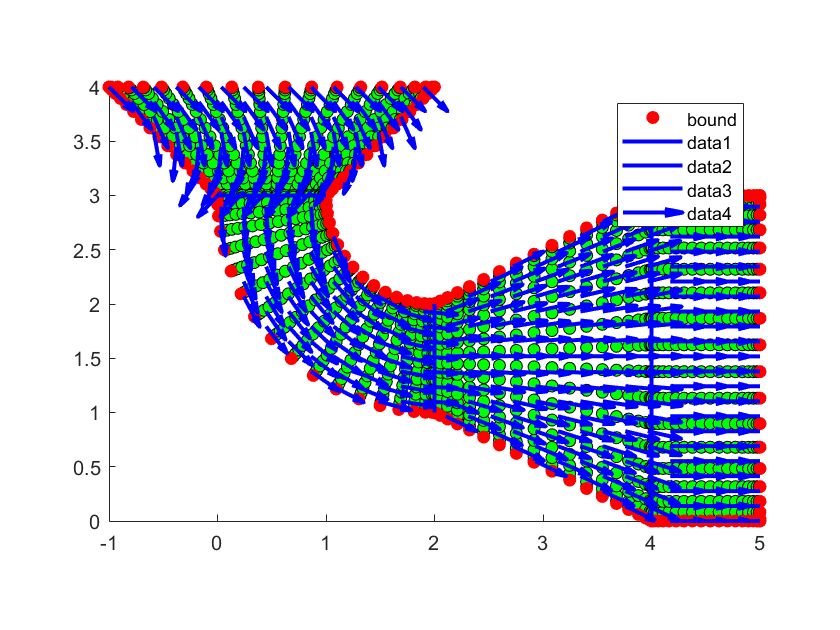
\includegraphics[scale=0.35]{F1.png}
%		\caption{Forward $\rho$ for $a = 0.01$} 
%		\label{F1}
%	\end{figure}

\begin{document}
\section*{Sedimentation}
\section{The Forward Model}
We are interested in modelling sedimentation processes. In order to achieve this, the advection-diffusion equation with mean-field interaction term has to be modified to include an approximation to volume exclusion. Archer and Malijevs\'y \cite{ArcherSed1} have achieved this using the following model to describe sedimentation processes. 
The modelling equations are:
\begin{align*}
	&\frac{\partial \rho}{\partial t^*} = \Gamma\nabla \cdot \left(  \rho \nabla \frac{\delta F[\rho]}{\delta \rho} \right) ,
\end{align*}
where $\Gamma$ is the diffusion coefficient. 	
We can rescale this equation as done in \cite{ArcherSed1} using the relationship $t = t^*/ \tau_B$, where $\tau_B = \beta \sigma^2 / \Gamma$ is the Brownian time scale.
Applying this rescaling we get:
\begin{align}\label{Eq1}
	&\frac{\partial \rho}{\partial t} = \beta \sigma^2\nabla \cdot \left(  \rho \nabla \frac{\delta F[\rho]}{\delta \rho} \right).
\end{align}
The free energy functional considered in \cite{ArcherSed1} is:
\begin{align*}
	F[\rho] &= \frac{1}{\beta} \int \rho (\ln \Lambda^2 \rho - 1) + f_{HDA} dr + \frac{1}{2}\int \int \rho(r) \rho(r') V_2(|r - r'|) dr dr' + \int \rho V_{ext} dr,
\end{align*}
where $f_{dh}$ the approximate free energy density describing the volume exclusion through hard disks. The external potential is defined as:
\begin{align*}
	V_{ext} &= c y, \quad \text{for } \quad 0 < y < L,
\end{align*}
where $c$ a constant and $L$ is the height of a rectangular domain. Outside these bounds $V_{ext} = \infty$. 
Furthermore, we have the pair potential:
\begin{align*}
	V_2 = exp(-r/\sigma),
\end{align*}
where $\sigma$ is the particle diameter of the hard sphere particle.


\subsection{The Hard Disk Approximation}
The part of the free energy functional, which accounts for the hard disk approximation, is:
\begin{align*}
	F_{HDA}[\rho] &= \frac{1}{\beta} \int  f_{HDA} dr = \frac{1}{\beta} \int   -  \rho - \rho \ln(1 - \eta) + \frac{\rho}{1 - \eta} dr,
\end{align*}
where $\eta = a \rho = \frac{\pi \sigma^2}{4} \rho$.
This can be thought of as the bulk fluid, one species, two dimensional approximation of Fundamental Measure Theory (FMT)  \cite{RosenfeldFMT}, which is a Density Functional Theory for hard sphere mixtures. The basis of this theory is that the excess free energy functional is of the form:
\begin{align*}
	\beta F_{ex}[{\rho_i}] = \int \Phi({n_\alpha(r')})d^3r',
\end{align*} 
where $i$ is the species count and $\Phi$ is a function of the weighted densities $n_\alpha$. By now there are many different versions of $\Phi$, yielding approximations of $F_{ex}$ with different limitations, see \cite{Roth_2010FMTReview}. Rosenfeld's original version is defined as:
	\begin{align*}
	\Phi = -n_0 \ln(1-n_3) + \frac{n_1 n_2 - \mathbf{n_1} \cdot \mathbf{n_2}}{1-n_3} + \frac{n_2^3 - 3n_2 \mathbf{n_2} \cdot \mathbf{n_2}}{24 \pi (1-n_3)^2}.
	\end{align*}
The weighted densities for $\nu$ species are:
	\begin{align} \label{eqn:WeightedDensities}
		n_\alpha (r) = \sum_{i=1}^\nu \int \rho_i(r') \omega_\alpha^i(r -r').
	\end{align}
The weight functions chosen by Rosenfeld are:
\begin{align*}
	&\omega_3^i = \Theta(R_i -r),\quad \omega_2^i = \delta(R_i -r),\quad \mathbf{\omega_2^i} = \frac{\mathbf r}{r}\delta (R_i -r),\quad \\
	&\omega_1^i = \omega_2^i/(4 \pi R_i), \quad \omega_0^i = \omega_2^i/(4\pi R_i^2), \quad \mathbf{\omega_1^i} = \mathbf{\omega_2^i}/(4 \pi R_i),
\end{align*}
where $R_i$ is the radius of the excluded volume, $\Theta$ is the Heaviside function and $\delta$ is the delta function. Integrating over $\omega_\alpha$, with $\alpha = 0,1,2,3$, we get the fundamental measures of a sphere: volume, surface area, radius and the Euler characteristic \cite{Roth_2010FMTReview} \cite{RosenfeldFMT}.
\\
Based on this theory for three dimensional spheres and the fact that the theory for hard rods is known exactly \cite{Percus1976}, Rosenfeld derived a version of this approach for two dimensional hard disks \cite{Rosenfeld2DInterp}. However, some additional approximations have to be made when choosing the weighted densities, which is not necessary in one and three dimensions. The resulting equation is:
\begin{align*}
	\Phi = - n_0 \ln(1-n_3) + \frac{1}{4 \pi} \frac{n_2 n_2}{1-n_3} + \frac{1}{4 \pi} \frac{\mathbf{n_2} \cdot \mathbf{n_2}}{1-n_3}.
\end{align*}
\\
In the uniform limit, for one particle species, we get that:
\begin{align*}
	n_0 = \rho, \quad n_2 = 2 \pi R \rho, \quad n_3 = \pi R^2 \rho,
\end{align*}
by solving the integrals in \eqref{eqn:WeightedDensities}, using spherical polar coordinates, with $\rho = \rho_{\text{bulk}}$, a constant. 
Substituting this in the 2D version of $\Phi$ gives:
\begin{align*}
	\Phi = - \rho \ln (1- \pi R^2 \rho) + \frac{1}{4 \pi} \frac{4\pi^2 R^2 \rho^2}{1 - \pi R^2 \rho} + \frac{1}{4 \pi}\frac{\mathbf{n_2} \cdot \mathbf{n_2}}{1 - \pi R^2 \rho},
\end{align*}
where $\mathbf{n_2} = \mathbf 0$ in the uniform limit, since the corresponding equation in \eqref{eqn:WeightedDensities} is an integral over an odd function.
Noting that $R = \sigma/2$ and $\eta = \pi \sigma^2 \rho /4$, we get that:
\begin{align*}
	\Phi = - \rho \ln (1- \eta) + \frac{\rho \eta}{1 - \eta} = \rho \left(\ln(1-\eta) + \frac{1}{1- \eta} -1 \right).
\end{align*} 
This expression for the free energy for the bulk fluid is the same as derived by scaled particle theory \cite{Reiss1959}, \cite{Reiss1960}, \cite{Helfand1961}, which also coincides with the Percus-Yevic compressibility equation \cite{PercusYevick1}, as detailed in \cite{RosenfeldSPT}.


\subsection{Deriving the equation of motion}
Since we are interested in the equation of motion, we need to calculate $ \nabla \cdot \left(\rho \nabla \frac{\delta F_{HDA}[\rho]}{\delta \rho} \right)$. We combine $F_{HDA}$ and $F_{ID}$ here so that we have:
\begin{align*}
	F_{N} = F_{HDA} + F_{ID}.
\end{align*}
Taking the functional derivative of $F_{N}$ gives:
\begin{align*}
	\frac{\delta F_{N}[\rho]}{\delta \rho} &= \frac{1}{\beta} \bigg(1 + \ln \rho + \Lambda^2 -2 - \ln(1-\eta) + a \frac{\rho}{1 - \eta} + \frac{1}{1 - \eta} + a \frac{\rho}{(1 - \eta)^2}  \bigg)\\
	&= \frac{1}{\beta} \bigg(1 + \ln \rho + \Lambda^2 -2 - \ln(1-\eta) + \frac{1}{(\eta - 1)^2} - \frac{1}{\eta - 1}  - 1\bigg)\\
	&= \frac{1}{\beta} \bigg( \ln \rho + \Lambda^2 - 2 - \ln(1-\eta) - \frac{\eta - 2}{(\eta - 1)^2}  \bigg),
\end{align*}
using partial fractions.
\begin{align*}
	\nabla \frac{\delta F_{N}[\rho]}{\delta \rho} &= \frac{1}{\beta} \bigg( \nabla\ln \rho + \nabla(\Lambda^2 - 2) - \nabla\ln(1-\eta) - \nabla\frac{\eta - 2}{(\eta - 1)^2}  \bigg)\\
	& = \frac{1}{\beta} \bigg( \frac{\nabla \rho}{\rho} - \frac{\nabla( 1- \eta)}{1 - \eta} - \nabla\frac{\eta - 2}{(\eta - 1)^2}  \bigg)\\
	& = \frac{1}{\beta} \bigg( \frac{\nabla \rho}{\rho} + \frac{\nabla \eta}{1 - \eta} - \nabla\frac{\eta - 2}{(\eta - 1)^2}  \bigg)
\end{align*}
Then multiplying by $\rho$ gives:
\begin{align*}
	\rho \nabla \frac{\delta F_{N}[\rho]}{\delta \rho} &= \frac{1}{\beta} \bigg( \nabla \rho +   \frac{\rho \nabla \eta}{1 - \eta} - \rho \nabla\frac{\eta - 2}{(\eta - 1)^2}  \bigg)\\
	&= \frac{1}{\beta} \bigg( \nabla \rho +   \frac{\eta\nabla \rho}{1 - \eta} - \rho \nabla\frac{\eta - 2}{(\eta - 1)^2}  \bigg)\\
	&= \frac{1}{\beta} \bigg( \nabla \rho + \frac{\nabla \rho}{1 - \eta} - \nabla \rho - \rho \nabla\frac{\eta - 2}{(\eta - 1)^2}  \bigg)\\
	&= \frac{1}{\beta} \bigg(  \frac{\nabla \rho}{1 - \eta}  - \rho \nabla\frac{\eta - 2}{(\eta - 1)^2}  \bigg)
\end{align*}
Finally we take the divergence:
\begin{align*}
	\nabla \cdot \bigg(\rho \nabla \frac{\delta F_{N}[\rho]}{\delta \rho}\bigg) &= \frac{1}{\beta} \bigg( \nabla  \cdot \left(  \frac{\nabla \rho}{1 - \eta} \right) - \nabla  \cdot \left(\rho \nabla\frac{\eta - 2}{(\eta - 1)^2} \right) \bigg)\\
	&= \frac{1}{\beta} \bigg( \frac{\nabla^2 \rho}{1 - \eta} +  \nabla \rho \cdot \nabla \frac{1}{1 - \eta} - \nabla \rho \cdot \nabla \frac{\eta - 2}{(\eta - 1)^2} - \rho \nabla^2\frac{\eta - 2}{(\eta - 1)^2} \bigg)\\
	&= \frac{1}{\beta} \bigg( \frac{\nabla^2 \rho}{1 - \eta} +  \nabla \rho \cdot \nabla \frac{(3- 2 \eta)}{(1 - \eta)^2}  - \rho \nabla^2\frac{\eta - 2}{(\eta - 1)^2} \bigg)
\end{align*}

\section{Optimality Conditions}
One optimal control problem to consider is:
\begin{align}\label{eq:OCP1}
	&J = \frac{1}{2}\int_0^T \int_\Omega (\rho - \widehat \rho)^2 dr dt + \frac{\beta}{2} \int_0^T\int_\Omega \w(r)^2 dr \notag\\
	&\text{subject to:}\\
	&\frac{\partial \rho}{\partial t} = \beta \sigma^2 \bigg( \nabla \cdot (\rho \nabla V_{ext}) - \nabla (\rho \w) + \nabla \cdot \left(\rho \nabla \frac{\delta F_{N}[\rho]}{\delta \rho}\right) + \kappa \int_\Omega \rho(r) \rho(r') \K(r,r')dr\bigg), \notag
\end{align}
where $\K(r,r') = \nabla V_2$.
We consider the terms of the PDE and the boundary conditions separately here.
\subsection{Calculating Frech\'et Derivatives}
In order to derive the optimalty conditions for the above OCP, we need to calculate the Frech\'et derivatives of the following terms:
\begin{align*}
	\nabla \cdot \bigg(\rho \nabla \frac{\delta F_{N}[\rho]}{\delta \rho}\bigg)
	&= \frac{1}{\beta} \bigg( \frac{\nabla^2 \rho}{1 - \eta} +  \nabla \rho \cdot \nabla \frac{(3- 2 \eta)}{(1 - \eta)^2}  - \rho \nabla^2\frac{\eta - 2}{(\eta - 1)^2} \bigg),
\end{align*}
where $\eta = a \rho$ and $a = \pi \sigma^2 /4$.
Consider:
\begin{align*}
	F_1(\rho) &= \nabla^2 \rho \frac{1}{1- a\rho},\\
	F_2(\rho) &= \nabla \rho \cdot \nabla \left(\frac{3-2a\rho}{(1-a\rho)^2}\right),\\
	F_3(\rho) &= \rho \nabla^2 \left(\frac{a\rho -2}{(a\rho -1)^2}\right).
\end{align*}
Then
\begin{align*}
	F_1(\rho + h) - F_1(\rho) &= \nabla (\rho +h) \frac{1}{1- a(\rho +h)} - \nabla \rho \frac{1}{1- a\rho}.
\end{align*}
Using the expansion: 
\begin{align*}
	\frac{1}{c - x} = \frac{1}{c} + \frac{1}{c^2}x + O(x^2),
\end{align*}
where $c = 1- a \rho$, we get:
\begin{align*}
	F_1(\rho + h) - F_1(\rho) &= \nabla^2 (\rho +h) \left(\frac{1}{1- a\rho} + \frac{a}{(1- a\rho)^2}h \right)- \nabla^2 \rho \frac{1}{1- a\rho}\\
	&= \nabla^2 h \left(\frac{1}{1- a\rho} \right) + \nabla^2 \rho \left(\frac{a}{(1- a\rho)^2}h\right),
\end{align*}
not considering higher order terms of $h$.
For $F_2$ we consider the expansion:
\begin{align*}
	\frac{1}{(c-x)^2} = \frac{1}{c^2} + \frac{2}{c^3}x + O(x^2),
\end{align*}
and get:
\begin{align*}
	F_2(\rho+h) - F_2(\rho) &= \nabla (\rho +h) \cdot \nabla \left(\frac{3-2a(\rho +h)}{(1-a(\rho+h))^2}\right) -\nabla \rho \cdot \nabla \left(\frac{3-2a\rho}{(1-a\rho)^2}\right) \\
	&= \nabla (\rho +h) \cdot \nabla \left(\frac{3-2a(\rho +h)}{(1-a\rho)^2} + \frac{3-2a(\rho +h)}{(1-a\rho)^3} 2ah \right) -\nabla \rho \cdot \nabla \left(\frac{3-2a\rho}{(1-a\rho)^2}\right)\\
	&=\nabla h \cdot \nabla \left(\frac{3-2a\rho}{(1-a\rho)^2} \right) + \nabla \rho \cdot \nabla \left(h\left(\frac{-2a }{(1-a\rho)^2} + \frac{6a-4a^2  \rho}{(1-a\rho)^3}  \right)\right)\\
	& = \nabla h \cdot \nabla \left( \frac{3-2a\rho}{(1-a\rho)^2} \right) + \left(\nabla h \cdot \nabla \rho \right) \left( \frac{-2a }{(1-a\rho)^2} + \frac{6a-4a^2  \rho}{(1-a\rho)^3}  \right) \\
	&+ h \nabla \rho \cdot \nabla \left(\frac{-2a }{(1-a\rho)^2} + \frac{6a-4a^2  \rho}{(1-a\rho)^3}  \right).
\end{align*}

Finally, we have:
\begin{align*}
	F_3(\rho+h) - F_3(\rho) &= (\rho +h) \nabla^2 \left(\frac{a(\rho +h) -2}{(a(\rho +h) -1)^2}\right) -\rho \nabla^2 \left(\frac{a\rho -2}{(a\rho -1)^2}\right)\\
	&=  (\rho +h) \nabla^2 \left(\frac{a(\rho +h) -2}{(1-a\rho)^2} + \frac{a(\rho +h) -2}{(1-a\rho)^3}2ah \right) -\rho \nabla^2 \left(\frac{a\rho -2}{(a\rho -1)^2}\right)\\
	&= h \nabla^2 \left(\frac{a\rho -2}{(a\rho -1)^2}\right) + \rho \nabla^2  \left(h\left(\frac{a }{(1-a\rho)^2} + \frac{2a^2\rho -4a}{(1-a\rho)^3} \right)\right)\\
	&= h \nabla^2 \left(\frac{a\rho -2}{(a\rho -1)^2}\right) + \rho  \left(\frac{a }{(1-a\rho)^2} + \frac{2a^2\rho -4a}{(1-a\rho)^3} \right)\nabla^2 h \\
	&+ 2 \rho \nabla \left(\frac{a }{(1-a\rho)^2} + \frac{2a^2\rho -4a}{(1-a\rho)^3} \right) \cdot \nabla h + \rho h \nabla^2  \left(\frac{a }{(1-a\rho)^2} + \frac{2a^2\rho -4a}{(1-a\rho)^3} \right).\\
\end{align*}
\subsection{Adjoint Equation}
In order to derive the adjoint equation, we need to consider the Lagrangian of the above OCP and take the derivative with respect to $\rho$. Given that most of the analysis has been done in a different chapter, we only consider the terms derived from $F_{N}$.
The Frech\'et derivatives of the relevant terms have been taken and are combined to give:
\begin{align*}
	\mathcal{L}_\rho(\rho,\w,q)h &= ... -\frac{1}{\beta}\int_0^T \int_\Omega q \nabla^2 h \left(\frac{1}{1- a\rho} \right) + q\nabla^2 \rho \left(\frac{a}{(1- a\rho)^2}h\right)\\
	&+ q\nabla h \cdot \nabla \left( \frac{3-2a\rho}{(1-a\rho)^2} \right) + q\left(\nabla h \cdot \nabla \rho \right) \left( \frac{-2a }{(1-a\rho)^2} + \frac{6a-4a^2  \rho}{(1-a\rho)^3}  \right) \\
	&+ qh \nabla \rho \cdot \nabla \left(\frac{-2a }{(1-a\rho)^2} + \frac{6a-4a^2  \rho}{(1-a\rho)^3}  \right)\\
	&- qh \nabla^2 \left(\frac{a\rho -2}{(a\rho -1)^2}\right) - q\rho  \left(\frac{a }{(1-a\rho)^2} + \frac{2a^2\rho -4a}{(1-a\rho)^3} \right)\nabla^2 h \\
	&- q\rho \nabla \left(\frac{2a }{(1-a\rho)^2} + \frac{4a^2\rho -8a}{(1-a\rho)^3} \right) \cdot \nabla h - q\rho h \nabla^2  \left(\frac{a }{(1-a\rho)^2} + \frac{2a^2\rho -4a}{(1-a\rho)^3} \right).
\end{align*}
Rearranging gives:
\begin{align*}
	\mathcal{L}_\rho(\rho,\w,q)h &=... -\frac{1}{\beta}\int_0^T \int_\Omega h \bigg(q\nabla^2 \rho \left(\frac{a}{(1- a\rho)^2}\right)  + q \nabla \rho \cdot \nabla \left(\frac{-2a }{(1-a\rho)^2} + \frac{6a-4a^2  \rho}{(1-a\rho)^3}  \right) - q \nabla^2 \left(\frac{a\rho -2}{(a\rho -1)^2}\right)\\
	&- q\rho  \nabla^2  \left(\frac{a }{(1-a\rho)^2} + \frac{2a^2\rho -4a}{(1-a\rho)^3} \right)\bigg)\\
	&+ \nabla h \cdot \bigg( q  \nabla \left( \frac{3-2a\rho}{(1-a\rho)^2} \right) + q \nabla \rho  \left( \frac{-2a }{(1-a\rho)^2} + \frac{6a-4a^2  \rho}{(1-a\rho)^3}  \right)- q\rho \nabla \left(\frac{2a }{(1-a\rho)^2} + \frac{4a^2\rho -8a}{(1-a\rho)^3} \right) \bigg)\\
	&+ \nabla^2 h \bigg(q \left(\frac{1}{1- a\rho} \right)  - q\rho  \left(\frac{a }{(1-a\rho)^2} + \frac{2a^2\rho -4a}{(1-a\rho)^3} \right)  \bigg).
\end{align*}
Integration by parts gives:
\begin{align*}
	\mathcal{L}_\rho(\rho,\w,q)h &=... -\frac{1}{\beta}\int_0^T \int_\Omega h \bigg(q\nabla^2 \rho \left(\frac{a}{(1- a\rho)^2}\right)  + q \nabla \rho \cdot \nabla \left(\frac{-2a }{(1-a\rho)^2} + \frac{6a-4a^2  \rho}{(1-a\rho)^3} \right) - q \nabla^2 \left(\frac{a\rho -2}{(a\rho -1)^2}\right)\\
	&- q\rho  \nabla^2  \left(\frac{a }{(1-a\rho)^2} + \frac{2a^2\rho -4a}{(1-a\rho)^3} \right)\bigg)\\
	&-  h \nabla \bigg( q  \nabla \left( \frac{3-2a\rho}{(1-a\rho)^2} \right) + q \nabla \rho  \left( \frac{-2a }{(1-a\rho)^2} + \frac{6a-4a^2  \rho}{(1-a\rho)^3}  \right)- q\rho \nabla \left(\frac{2a }{(1-a\rho)^2} + \frac{4a^2\rho -8a}{(1-a\rho)^3} \right) \bigg)\\
	&+  h \nabla^2\bigg(q \left(\frac{1}{1- a\rho} \right)  - q\rho  \left(\frac{a }{(1-a\rho)^2} + \frac{2a^2\rho -4a}{(1-a\rho)^3} \right)  \bigg).
\end{align*}
So we have:
\begin{align*}
	\mathcal{L}_\rho(\rho,\w,q)h &=... -\frac{1}{\beta}\int_0^T\int_\Omega h \bigg[  q\nabla^2 \rho \left(\frac{a}{(1- a\rho)^2}\right)  + q \nabla \rho \cdot \nabla \left(\frac{-2a }{(1-a\rho)^2}+ \frac{6a-4a^2  \rho}{(1-a\rho)^3}  \right) - q \nabla^2 \left(\frac{a\rho -2}{(a\rho -1)^2}\right)\\
	&- q\rho  \nabla^2  \left(\frac{a }{(1-a\rho)^2} \right) - q\rho  \nabla^2  \left(\frac{2a^2\rho -4a}{(1-a\rho)^3} \right)\\
	& -\nabla \cdot \left( q  \nabla \left( \frac{3-2a\rho}{(1-a\rho)^2} \right) \right) - \nabla \cdot \left( q \nabla \rho  \left( \frac{-2a }{(1-a\rho)^2} \right)\right)  - \nabla \cdot \left( q \nabla \rho  \left(\frac{6a-4a^2  \rho}{(1-a\rho)^3}  \right)\right)  \\
	& + \nabla \cdot\left( q\rho \nabla \left(\frac{2a }{(1-a\rho)^2} \right) \right) + \nabla \cdot\left( q\rho \nabla \left( \frac{4a^2\rho -8a}{(1-a\rho)^3} \right) \right)\\
	&+   \nabla^2 \left(q \left(\frac{1}{1- a\rho} \right) \right) - \nabla^2 \left(q\rho  \left(\frac{a }{(1-a\rho)^2}\right)\right) - \nabla^2 \left(q\rho \left(\frac{2a^2\rho -4a}{(1-a\rho)^3} \right)\right)\bigg] dr dt .
\end{align*}
Combining fractions gives:
\begin{align*}
	\mathcal{L}_\rho(\rho,\w,q)h &=... -\frac{1}{\beta}\int_0^T\int_\Omega h \bigg[  q\nabla^2 \rho \left(\frac{a}{(1- a\rho)^2}\right)  + q \nabla \rho \cdot \nabla \left(\frac{2a(a \rho -2)}{(1-a\rho)^3} \right) - q \nabla^2 \left(\frac{a\rho -2}{(a\rho -1)^2}\right)\\
	& - q\rho  \nabla^2  \left(\frac{a(3  - a \rho)}{(1-a\rho)^3} \right) -\nabla \cdot \left( q  \nabla \left( \frac{3-2a\rho}{(1-a\rho)^2} \right) \right)  - \nabla \cdot \left( q \nabla \rho  \left(\frac{2a(a \rho -2)}{(1-a\rho)^3}  \right)\right)  \\
	&  + \nabla \cdot\left( q\rho \nabla \left( \frac{-2a(a \rho- 3)}{(1-a\rho)^3} \right) \right)+   \nabla^2 \left(q \left(\frac{1}{1- a\rho} \right) \right) - \nabla^2 \left(q\rho \left(\frac{-a(a \rho -3)}{(1-a\rho)^3} \right)\right)\bigg] dr dt. 
\end{align*}
According to Mathematica this is:
\begin{align*}
	\mathcal{L}_\rho(\rho,\w,q)h &=... -\frac{1}{\beta}\int_0^T\int_\Omega h \bigg[ 
	\frac{1}{(a \rho -1)^3}\bigg(4 a \nabla \rho \cdot \nabla q + 
	2 a (-1 + a \rho) q \nabla^2 \rho + (-1 + 5 a \rho - 2 a^2 \rho^2) \nabla^2 q\bigg)
	\bigg] dr dt.
\end{align*}
And rewriting this is:
\begin{align*}
	\mathcal{L}_\rho(\rho,\w,q)h & =... -\frac{1}{\beta}\int_0^T\int_\Omega h \bigg[ 
	\frac{4 a \nabla \rho \cdot \nabla q}{(a \rho -1)^3}  +   \frac{2 a  q \nabla^2 \rho}{(a \rho -1)^2}  +   \frac{(-1 + 5 a \rho - 2 a^2 \rho^2) \nabla^2 q}{(a \rho -1)^3}
	\bigg] dr dt.
\end{align*}
Adding the other terms of the adjoint found in previous analysis, the adjoint equation is:
\begin{align*}
	\frac{\partial q}{\partial t} =&\frac{1}{\beta}\frac{(-1 + 5 a \rho - 2 a^2 \rho^2) }{(a \rho -1)^3}\nabla^2 q +\frac{1}{\beta} \frac{4 a \nabla \rho }{(a \rho -1)^3}\cdot \nabla q +  \frac{1}{\beta} \frac{2 a   \nabla^2 \rho}{(a \rho -1)^2} q    \\
	&- \w \cdot \nabla q + \nabla V_{ext} \cdot \nabla q - \rho + \hr + \int \left(\nabla_r q(r) - \nabla_{r'} q(r') \right) \rho(r'). \K(r,r') dr'
\end{align*}


\subsection{Frech\'et Derivatives for Boundary Terms}
When considering no-flux boundary conditions, we have the equation:
\begin{align*}
	- \mathbf{j} \cdot \n = ... -\rho \nabla \frac{\delta F_{N}[\rho]}{\delta \rho} \cdot \n &= ...-\frac{1}{\beta} \bigg(  \frac{\nabla \rho}{1 - \eta}  - \rho \nabla\frac{\eta - 2}{(\eta - 1)^2}  \bigg) \cdot \n,
\end{align*}
omitting the other terms, as done in the previous section.
The Frech\'et derivatives of the following terms have to be taken, similarly to the section above:
\begin{align*}
	F_4(\rho) &= \frac{\nabla \rho}{1 - a \rho},\\
	F_5(\rho) &= \rho \nabla\frac{a \rho - 2}{(a \rho - 1)^2} .
\end{align*}
Then for $F_4$ we have:
\begin{align*}
	F_4(\rho+h) - F_4(\rho) &=\nabla (\rho + h) \frac{1}{1 - a (\rho + h)} - \nabla \rho \frac{1}{1 - a \rho}\\
	&= \nabla(\rho + h) \left(\frac{1}{1 - a\rho} + \frac{a}{(1 -a \rho)^2}h \right)\\
	&= \nabla h \left(\frac{1}{1 - a\rho}\right) + \nabla \rho \left( \frac{a}{(1 -a \rho)^2}h \right).
\end{align*}
For $F_5$ we get:
\begin{align*}
	F_5(\rho + h) - F_5(\rho) &= (\rho + h) \nabla\frac{a (\rho +h) - 2}{(a (\rho +h) - 1)^2}  - \rho \nabla\frac{a \rho - 2}{(a \rho - 1)^2} \\
	&=(\rho + h) \nabla \left( \frac{a (\rho +h) - 2}{(1- a \rho)^2} + \frac{a (\rho +h) - 2}{(1- a \rho)^3} 2ah\right) - \rho \nabla\frac{a \rho - 2}{(a \rho - 1)^2} \\
	&= h \nabla \left(\frac{a \rho  - 2}{(1- a \rho)^2}\right) + \rho \nabla \left( h\left( \frac{a}{(1- a \rho)^2} + \frac{2a^2\rho - 4a}{(1- a \rho)^3} \right)\right)\\
	&= h \nabla \left(\frac{a \rho  - 2}{(1- a \rho)^2}\right) + h \rho \nabla \left( \frac{a}{(1- a \rho)^2} + \frac{2a^2\rho - 4a}{(1- a \rho)^3} \right) + \nabla h \left( \rho \frac{a}{(1- a \rho)^2} + \rho\frac{2a^2\rho - 4a}{(1- a \rho)^3} \right).
\end{align*}
\subsection{Boundary Terms}
Given the Frech\'et derivatives, the relevant boundary terms for the Lagrangian are:
\begin{align*}
	\mathcal{L}_{\rho,1}(\rho,\w, q) h &=.. - \frac{1}{\beta}\int_0^T \int_{\partial \Omega} \bigg(- q_{\partial \Omega}\nabla h \left(\frac{1}{1 - a\rho}\right) - q_{\partial \Omega}\nabla \rho \left( \frac{a}{(1 -a \rho)^2}h \right)+ q_{\partial \Omega}h \nabla \left(\frac{a \rho  - 2}{(1- a \rho)^2}\right) \\
	&+ h q_{\partial \Omega}\rho \nabla \left( \frac{a}{(1- a \rho)^2} + \frac{2a^2\rho - 4a}{(1- a \rho)^3} \right) + q_{\partial \Omega}\nabla h \left( \rho \frac{a}{(1- a \rho)^2} + \rho\frac{2a^2\rho - 4a}{(1- a \rho)^3} \right) \bigg) \cdot \n dr. dt
\end{align*}

From the integration by parts of the terms within the domain (in the previous section) we get:
\begin{align*}
	\mathcal{L}_{\rho,2}(\rho, \w,q)h &=... - \frac{1}{\beta}\int_0^T \int_{\partial \Omega} \bigg(h \bigg( q  \nabla \left( \frac{3-2a\rho}{(1-a\rho)^2} \right) + q \nabla \rho  \left( \frac{-2a }{(1-a\rho)^2} + \frac{6a-4a^2  \rho}{(1-a\rho)^3}  \right)\\
	&- q\rho \nabla \left(\frac{2a }{(1-a\rho)^2} + \frac{4a^2\rho -8a}{(1-a\rho)^3} \right) \bigg)\\
	& + \nabla h \bigg(q \left(\frac{1}{1- a\rho} \right)  - q\rho  \left(\frac{a }{(1-a\rho)^2} + \frac{2a^2\rho -4a}{(1-a\rho)^3} \right)  \bigg) \\
	&- h \nabla \bigg(q \left(\frac{1}{1- a\rho} \right)  - q\rho  \left(\frac{a }{(1-a\rho)^2} + \frac{2a^2\rho -4a}{(1-a\rho)^3} \right)  \bigg) \bigg)\cdot \n dr dt.
\end{align*}


Combining all of these give all boundary terms for the Lagrangian:
\begin{align*}
	\mathcal{L}_\rho (\rho,\w,q)h &=... - \frac{1}{\beta}\int_0^T \int_{\partial \Omega} \bigg( h \bigg(-  q_{\partial \Omega}\nabla \rho \left( \frac{a}{(1 -a \rho)^2} \right)+ q_{\partial \Omega} \nabla \left(\frac{a \rho  - 2}{(1- a \rho)^2}\right) \\
	&+  q_{\partial \Omega}\rho \nabla \left( \frac{a}{(1- a \rho)^2} + \frac{2a^2\rho - 4a}{(1- a \rho)^3} \right)
	+ \bigg( q  \nabla \left( \frac{3-2a\rho}{(1-a\rho)^2} \right) + q \nabla \rho  \left( \frac{-2a }{(1-a\rho)^2} + \frac{6a-4a^2  \rho}{(1-a\rho)^3}  \right)\\
	&- q\rho \nabla \left(\frac{2a }{(1-a\rho)^2} + \frac{4a^2\rho -8a}{(1-a\rho)^3} \right) \bigg) -  \nabla \bigg(q \left(\frac{1}{1- a\rho} \right)  - q\rho  \left(\frac{a }{(1-a\rho)^2} + \frac{2a^2\rho -4a}{(1-a\rho)^3} \right)  \bigg)	\bigg)\\
	& +\nabla h \bigg(- q_{\partial \Omega} \left(\frac{1}{1 - a\rho}\right) + q_{\partial \Omega}\left( \rho \frac{a}{(1- a \rho)^2} + \rho\frac{2a^2\rho - 4a}{(1- a \rho)^3} \right) +q \left(\frac{1}{1- a\rho} \right) \\
	& - q\rho  \left(\frac{a }{(1-a\rho)^2} + \frac{2a^2\rho -4a}{(1-a\rho)^3} \right)  \bigg) \bigg) \cdot \n dr dt.
\end{align*}
Comparing terms in $\nabla h$:
\begin{align*}
	&\bigg[-q_{\partial \Omega} \left(\frac{1}{1 - a\rho}\right) + q_{\partial \Omega}\left( \rho \frac{a}{(1- a \rho)^2} + \rho\frac{2a^2\rho - 4a}{(1- a \rho)^3} \right) \\
	&+q \left(\frac{1}{1- a\rho} \right)  - q\rho  \left(\frac{a }{(1-a\rho)^2} + \frac{2a^2\rho -4a}{(1-a\rho)^3} \right) \bigg] \cdot \n = 0.
\end{align*}
This holds when $q_{\partial \Omega} = q$.
Then for $h \neq 0$ we get:
\begin{align*}
	&\bigg[-q\nabla \rho \left( \frac{a}{(1 -a \rho)^2} \right)+q \nabla \left(\frac{a \rho  - 2}{(1- a \rho)^2}\right) \\
	&+q\rho \nabla \left( \frac{a}{(1- a \rho)^2} + \frac{2a^2\rho - 4a}{(1- a \rho)^3} \right)
	+  q  \nabla \left( \frac{3-2a\rho}{(1-a\rho)^2} \right) + q \nabla \rho  \left( \frac{-2a }{(1-a\rho)^2} + \frac{6a-4a^2  \rho}{(1-a\rho)^3}  \right)\\
	&- q\rho \nabla \left(\frac{2a }{(1-a\rho)^2} + \frac{4a^2\rho -8a}{(1-a\rho)^3} \right) -  \nabla \bigg(q \left(\frac{1}{1- a\rho} \right)  - q\rho  \left(\frac{a }{(1-a\rho)^2} + \frac{2a^2\rho -4a}{(1-a\rho)^3} \right) \bigg)\bigg] \cdot \n = 0
\end{align*}
According to Mathematica this reduces to:
\begin{align*}
	\frac{(1 + a \rho) \nabla q}{(a \rho -1)^3}\cdot \n = 0
\end{align*}
Since $a \rho >0$ by definition, this is:
\begin{align*}
	\frac{\partial q}{\partial n} = 0.
\end{align*}
Note that the other terms of the PDE are not entering this expression, as they cancel out during the derivation. This has been shown in the derivation of a simpler set of equations and since this derivation is additive, the result remains unchanged.\\
Furthermore, the gradient equation remains unchanged by this equation, since $F_N$ does not contain terms involving $\w$, compare to \eqref{eqn:LwGradientEqn}, and is:
\begin{align*}
	\w = - \frac{1}{\beta}\rho \nabla q.
\end{align*}
\subsection{Time-Independent Control}
While the gradient equation is unchanged by the sedimentation equation, as compared to an advection diffusion equation, it is changed when we consider a time independent control.
We choose the problem:
\begin{align*}
	&J = \frac{1}{2}\int_0^T \int_\Omega (\rho - \widehat \rho)^2 dr dt + \frac{\beta}{2} \int_\Omega \w(r)^2 dr\\
	&\text{subject to:}\\
	&\frac{\partial \rho}{\partial t} = \beta \sigma^2 \bigg( \nabla \cdot (\rho \nabla V_{ext}) - \nabla (\rho \w) + \nabla \cdot \left(\rho \nabla \frac{\delta F_{N}[\rho]}{\delta \rho}\right) + \kappa \int_\Omega \rho(r) \rho(r') \K(r,r')dr\bigg),
\end{align*}
where $\K(r,r') = \nabla V_2$.
Taking derivatives of the Lagrangian with respect to $\w$ gives:
\begin{align}\label{eqn:LwGradientEqn}
	\mathcal{L}_\w(\rho,\w, q)h &= \int_\Omega \beta \w(r) \cdot \h(r) dt + \int_0^T \int_\Omega \rho \h(r) \cdot \nabla q dr dt.
\end{align}
Since $\w$ does not depend on $t$, neither does $\h$ and so this can be taken out of the time integral:
\begin{align*}
	\mathcal{L}_\w(\rho,\w, q)h &= \int_\Omega \bigg( \beta \w(r) \cdot \h(r)  + \h(r) \cdot \int_0^T \rho  \nabla q dt \bigg) dr.
\end{align*}
Then we get:
\begin{align*}
	\beta \w(r)  +  \int_0^T \rho  \nabla q dt = 0,
\end{align*}
and finally:
\begin{align*}
	\w(r) = - \frac{1}{\beta} \int_0^T \rho  \nabla q dt.
\end{align*}
\subsection{Periodic Boundary Conditions}
+++ Add here when done +++
\section{Numerical Results}
In this section, the results in \cite{ArcherSed1} are replicated. Then optimal control problems of the form \eqref{eq:OCP1} are solved.

\subsection{Replicating examples from the paper in a box with noflux BCs}
The domain in \cite{ArcherSed1} is a box with lengths $L_y = 43.5 \sigma$, and $L_x = 60 \sigma$. 
The strength of the external potential is given by $\beta c = 0.1$ and the strength of the interaction term $\kappa$ is given by $\beta \kappa = - 3.5$, where $\beta = \frac{1}{k_BT}$. 
Furthermore, we have the average density of the system $\bar \rho \sigma^2$, calculated using $(1/L_y)\int_0^L \rho \sigma^2 dy$.
The initial condition for $\rho$ is found by considering $\bar \rho$ and adding a uniform random number to each location in the range $\pm \bar \rho/ 20$. The cases $\sigma \bar \rho = 0.072$ and $\sigma \bar \rho = 0.2$ are considered in \cite{ArcherSed1}.
%Note that in this section we haven't applied the rescaling with $\sigma^2$ from Equation \eqref{Eq1} and so we cannot compare the time scale here with the one from the paper when considering $\sigma \neq 1$.
%\subsubsection{Example Figure 8}
%
%For simplicity, set $\beta = 1$ everywhere. Then set $\sigma = 1$, which gives for the example in Figure 8 that $\bar \rho = 0.072$. However, the domain is rescaled, such that $L_y = 21$, $L_x = 30$ but $\bar \rho = 0.072$. We further have $\kappa = - 3.5$, $a = 0.1$
%The number of points are $n = 30$, $N = 40$ and we run this up to time $T = 30$. If we were to instead increase the strength of $V_{ext}$, we would see the sediment flatten out more at the bottom. The result, which takes $12$ seconds to run, can be seen in Figure \ref{F1}. 
%\begin{figure}[h]
%	\centering
%	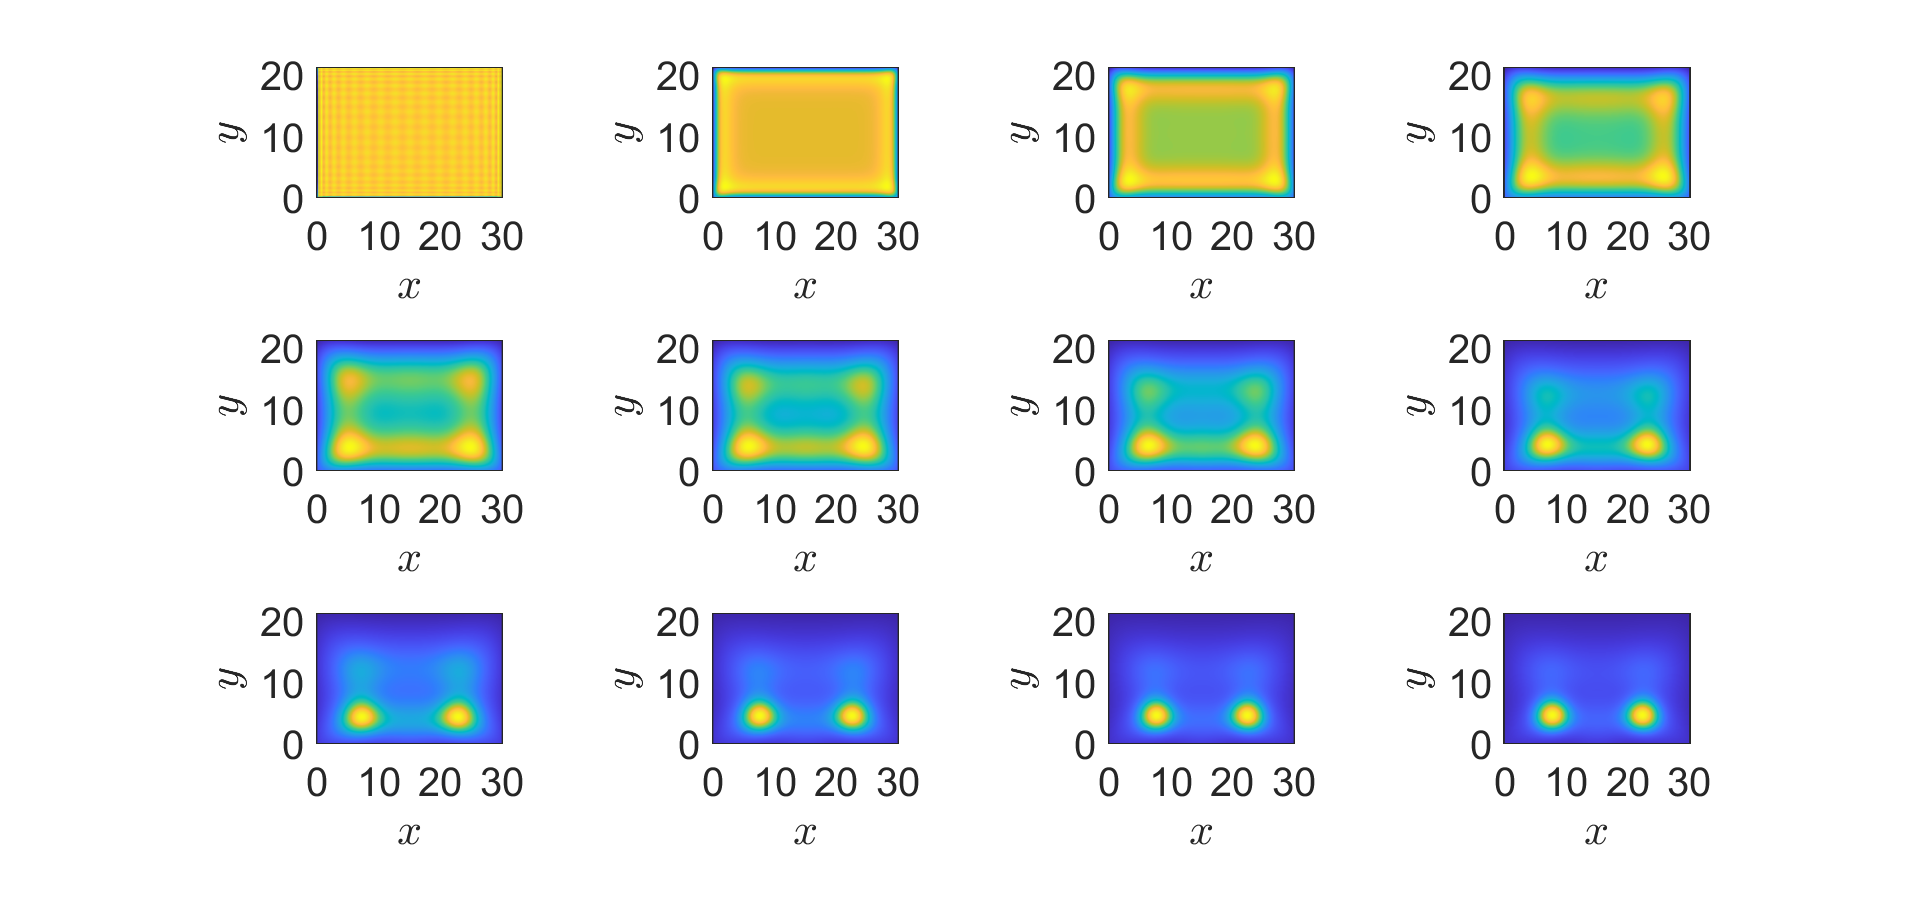
\includegraphics[scale=0.35]{Ex8F1.png}
%	\caption{Figure 8 Example, $\bar \rho = 0.072$, $\sigma = 1$, $12$ different times} 
%	\label{F1}
%\end{figure} 
%
%
%
%Next, we decrease $\sigma$ to get closer to the scaling from the paper. We set $\sigma = 0.8$. Inspecting the result, it is clear that it needs more points, so we run it with $N = 50$ instead. This increases running time from $30$ seconds to $2$ min. In Figure \ref{F2} we can see that a third cluster is building. 
%\begin{figure}[h]
%	\centering
%	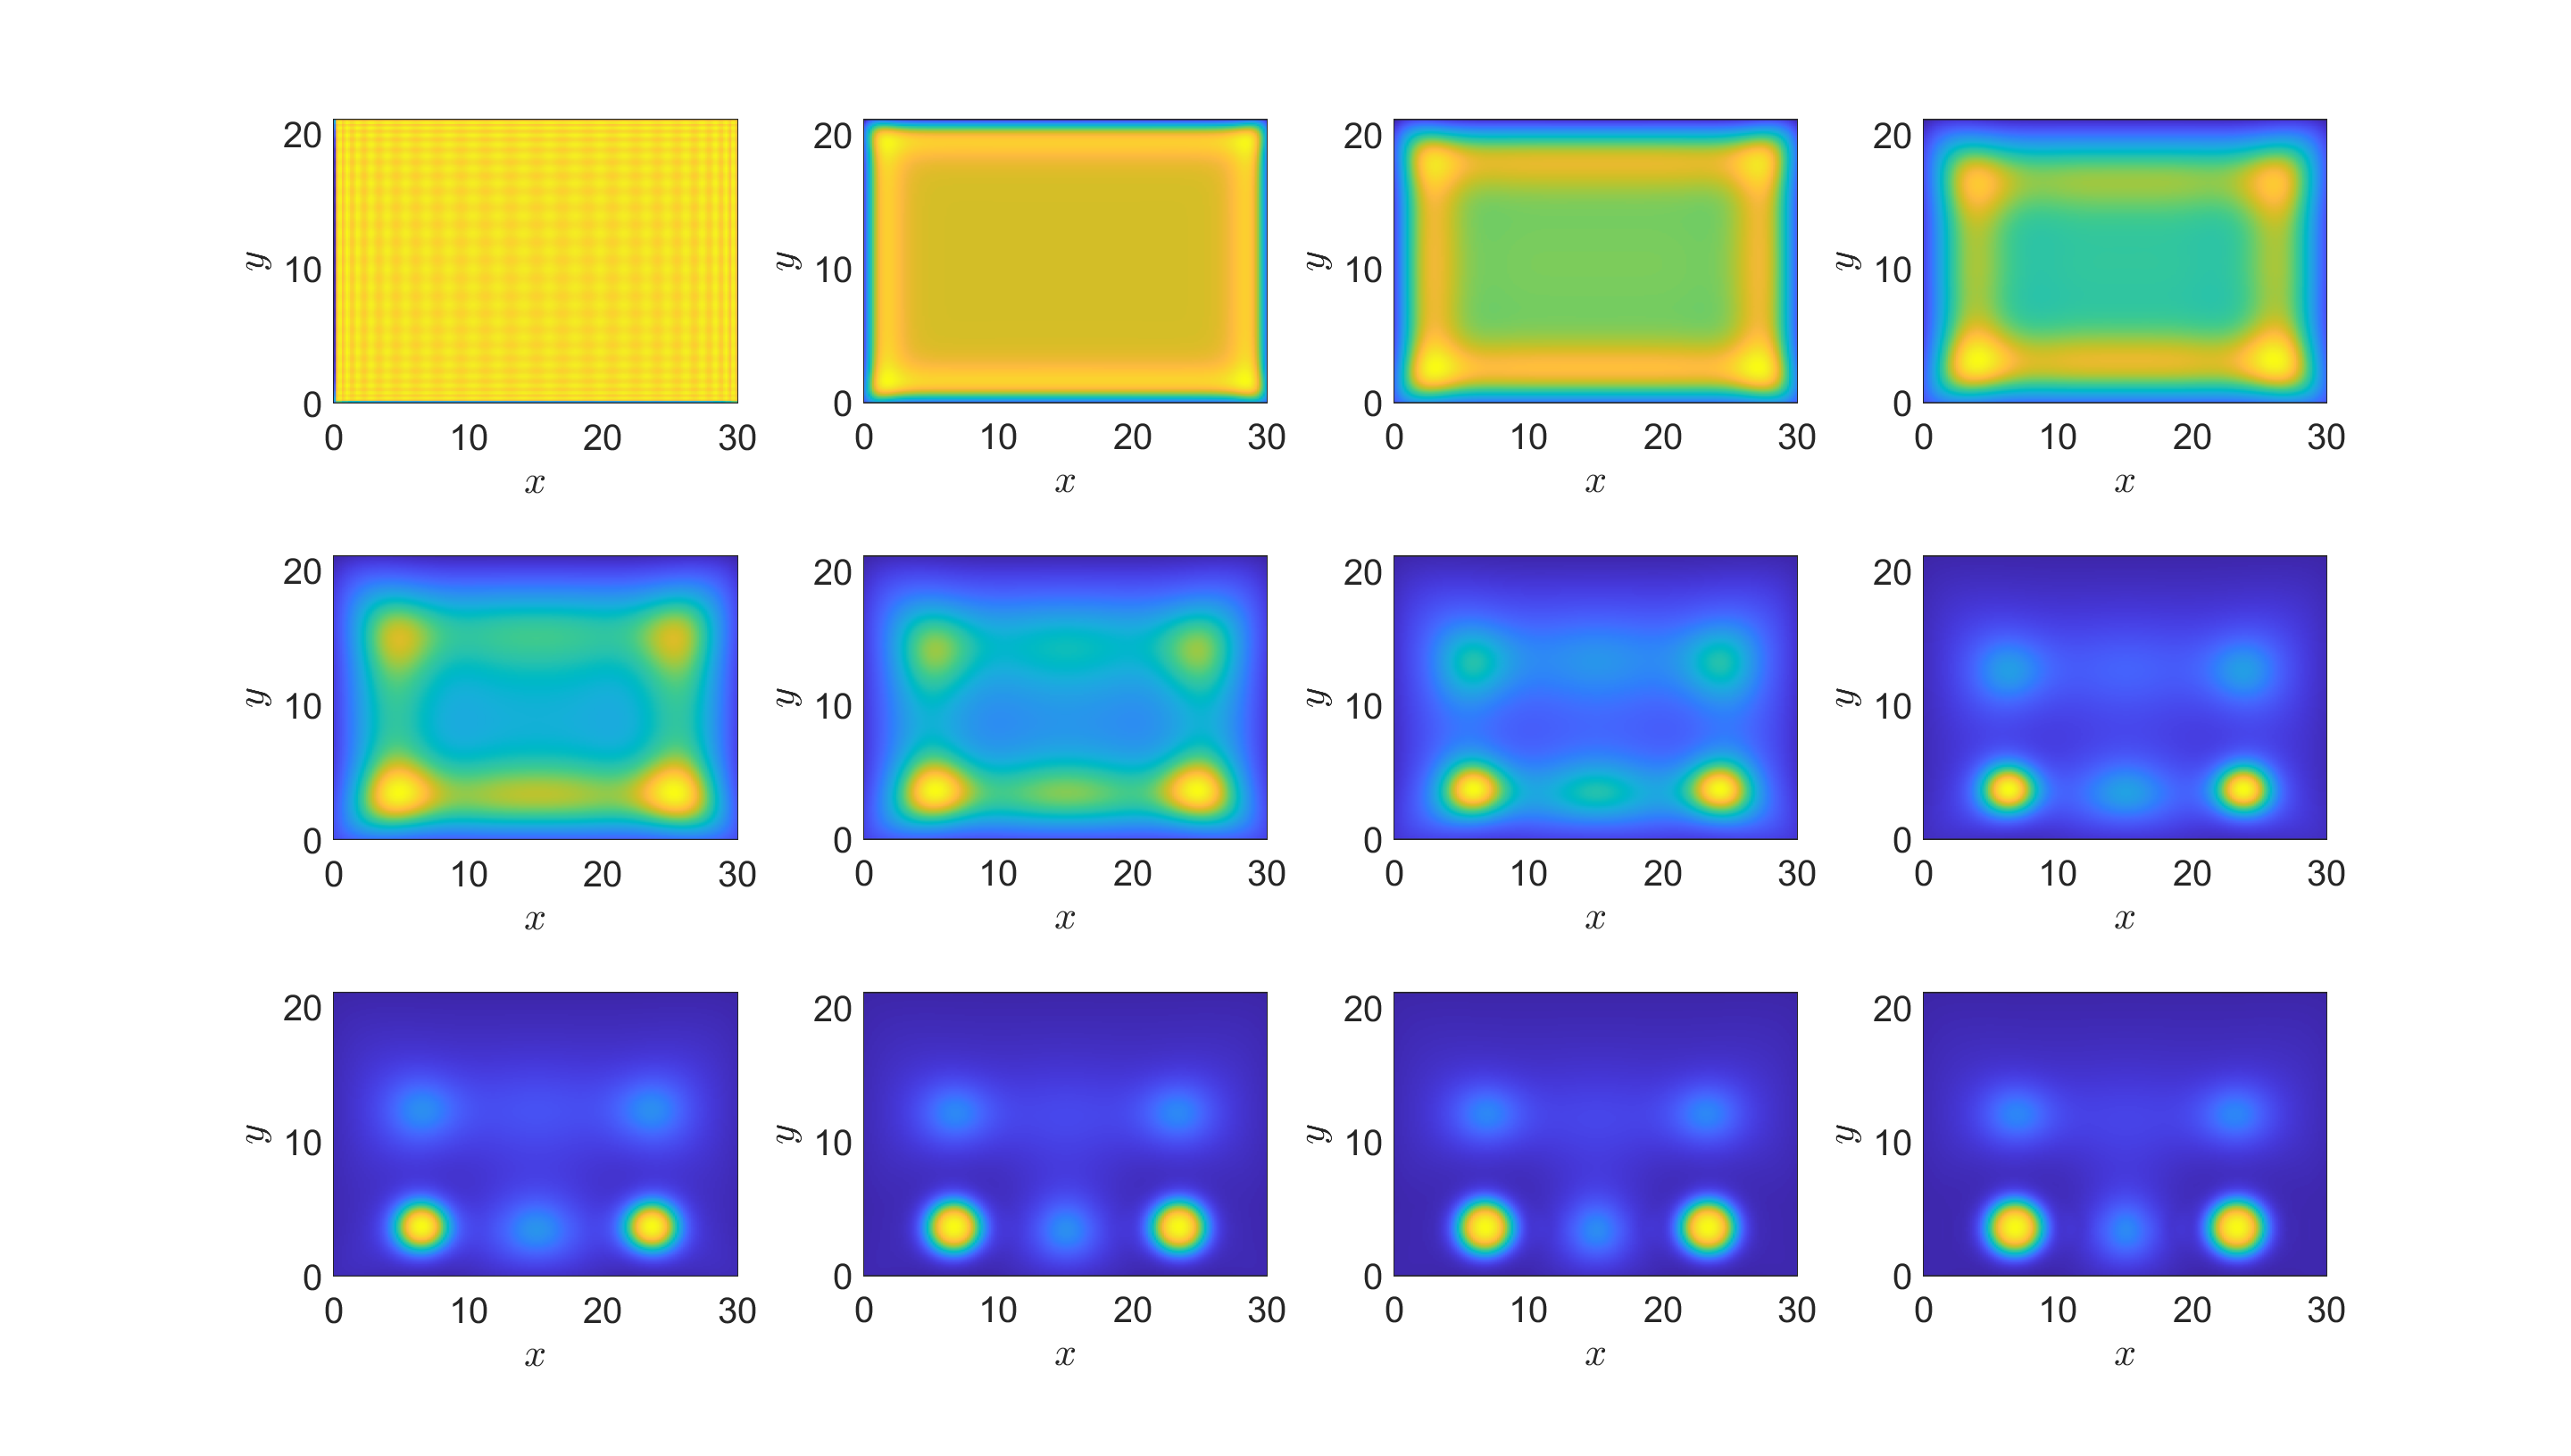
\includegraphics[scale=0.25]{Ex8F2.png}
%	\caption{Figure 8 Example, $\bar \rho = 0.072$, $\sigma = 0.8$, $12$ different times} 
%	\label{F2}
%\end{figure} 
%If we decrease $\sigma$ to $0.6$ we again need more points. We try $N = 60$, which takes $14$ min, but the result is still numerically unstable. This can be seen in Figure \ref{F3}.This configuration is closest to the actual model setup because we have half of the domain that Archer has, so we need to half $\sigma$.
%\begin{figure}[h]
%	\centering
%	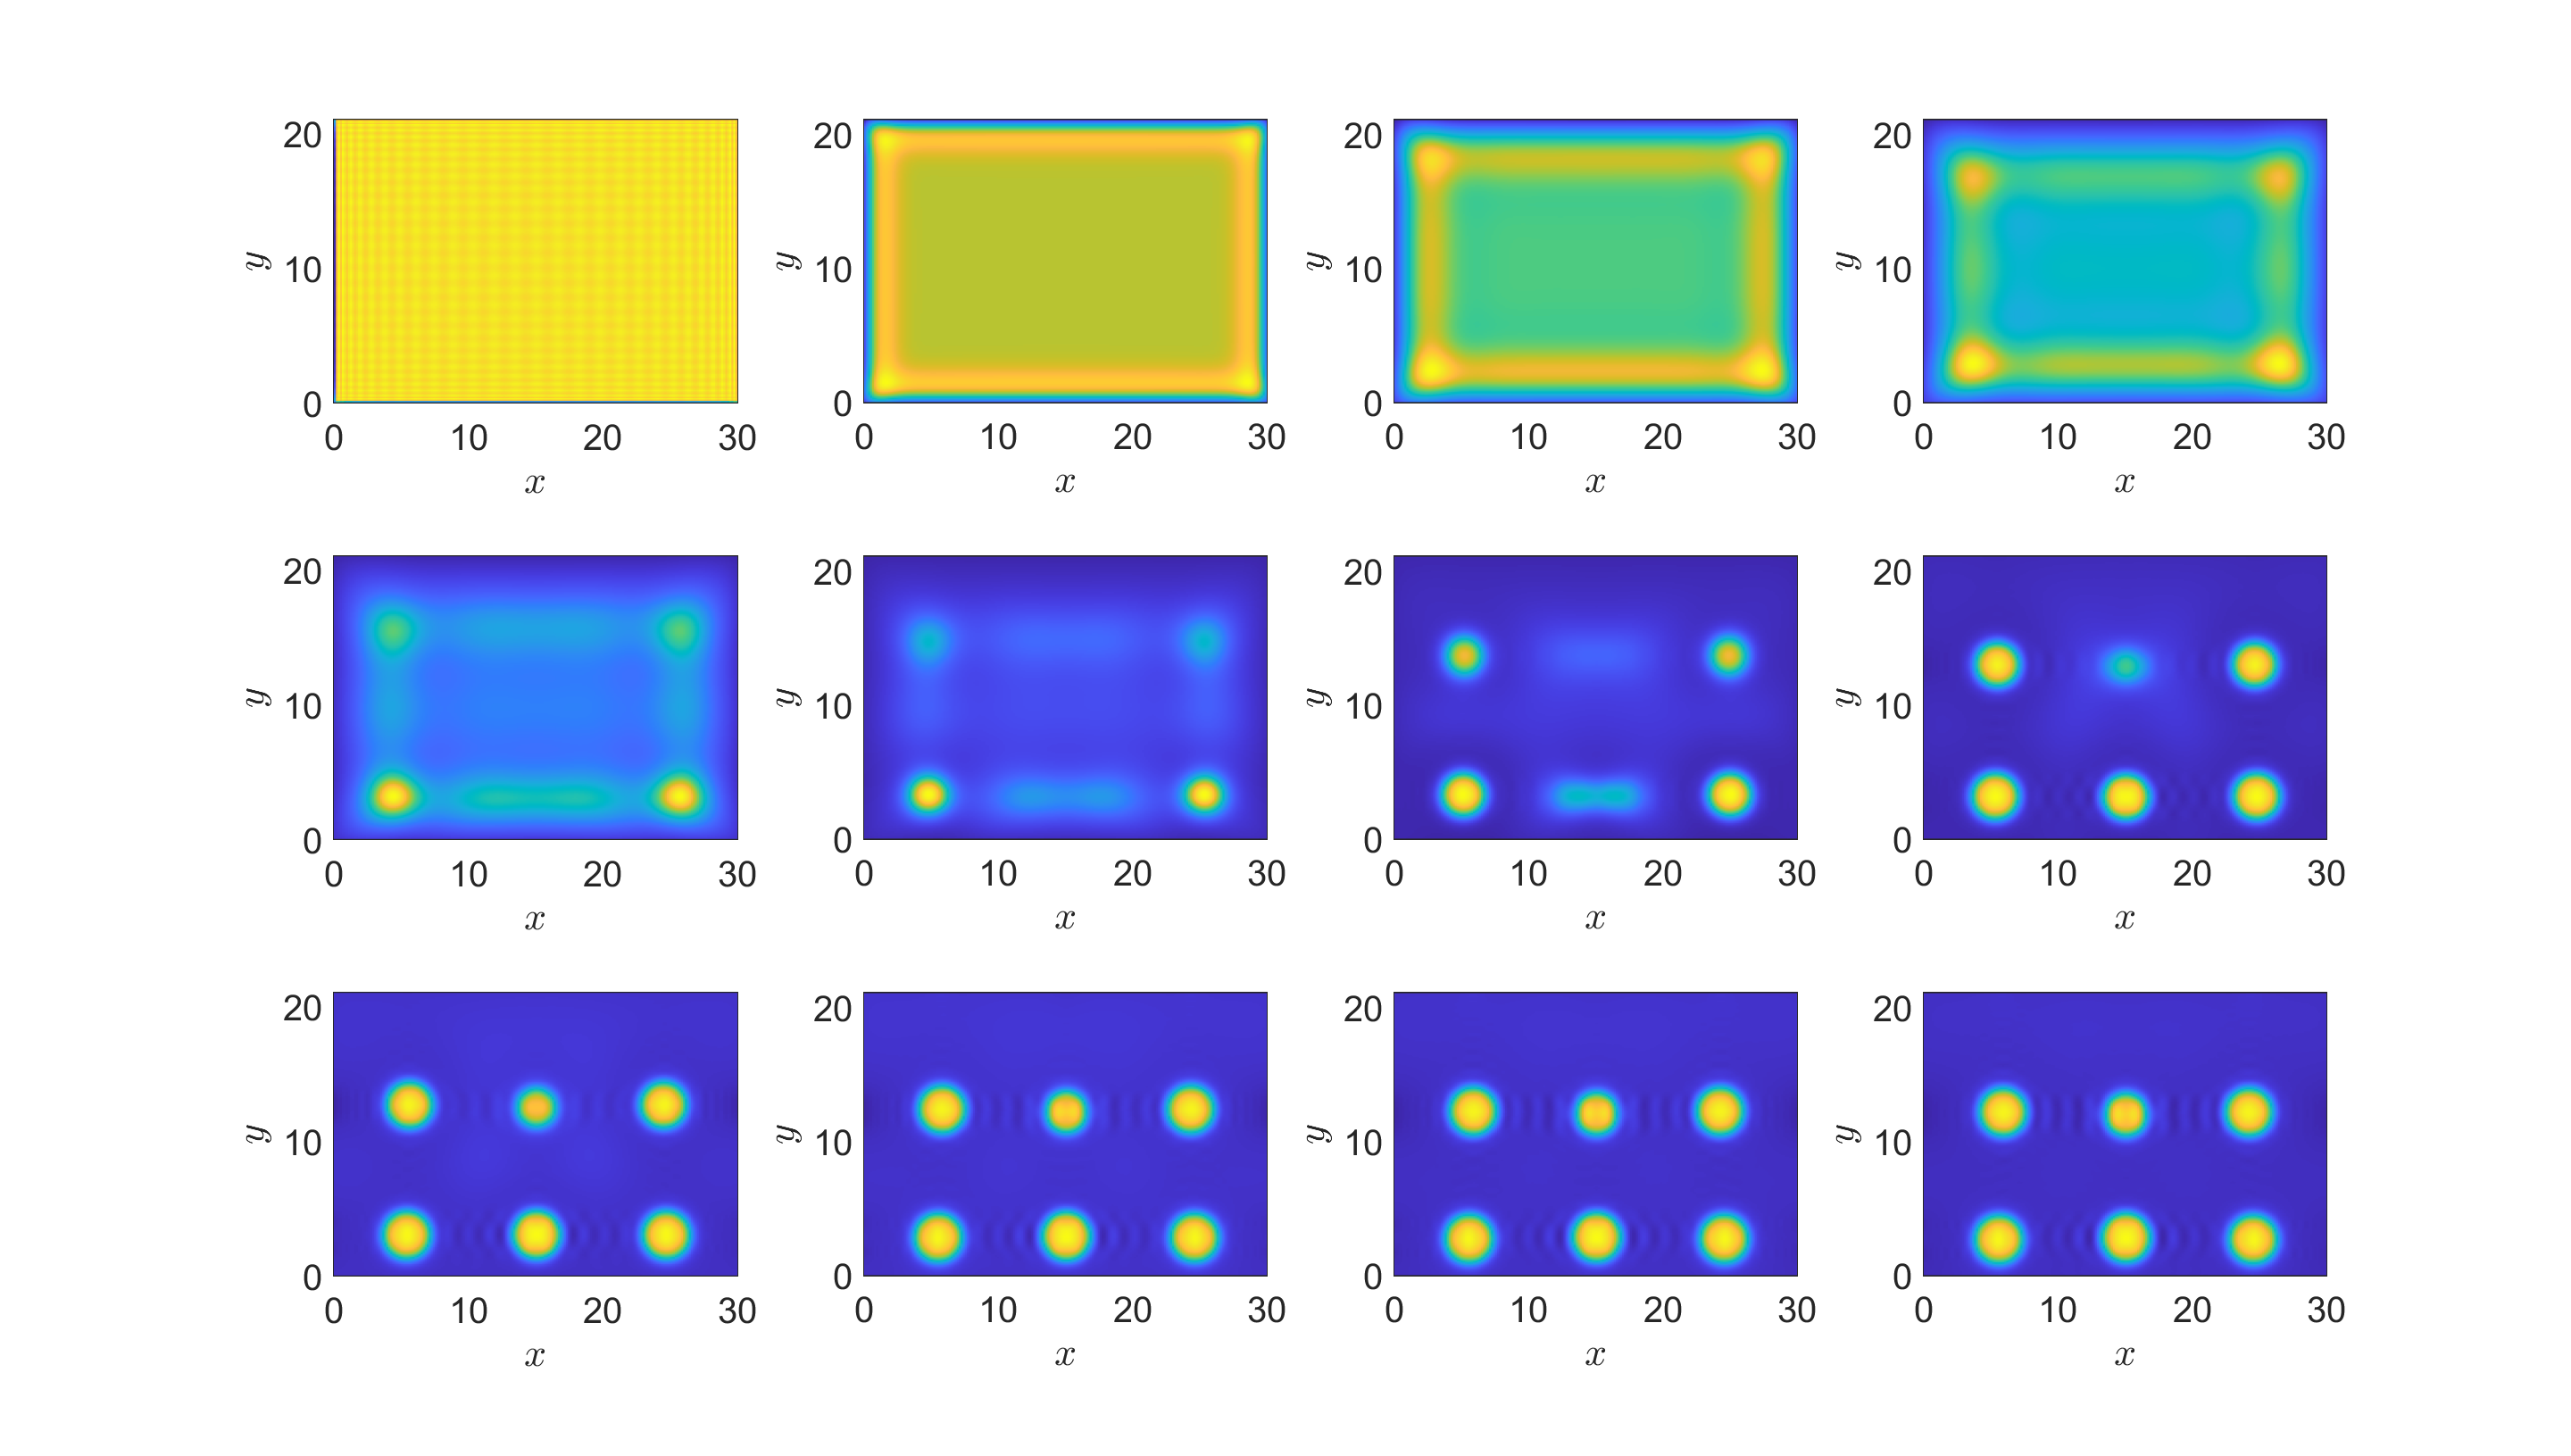
\includegraphics[scale=0.25]{Ex8F3.png}
%	\caption{Figure 8 Example, $\bar \rho = 0.072$, $\sigma = 0.5$, $12$ different times} 
%	\label{F3}
%\end{figure} 
%
%
%\begin{figure}[h]
%	\centering
%	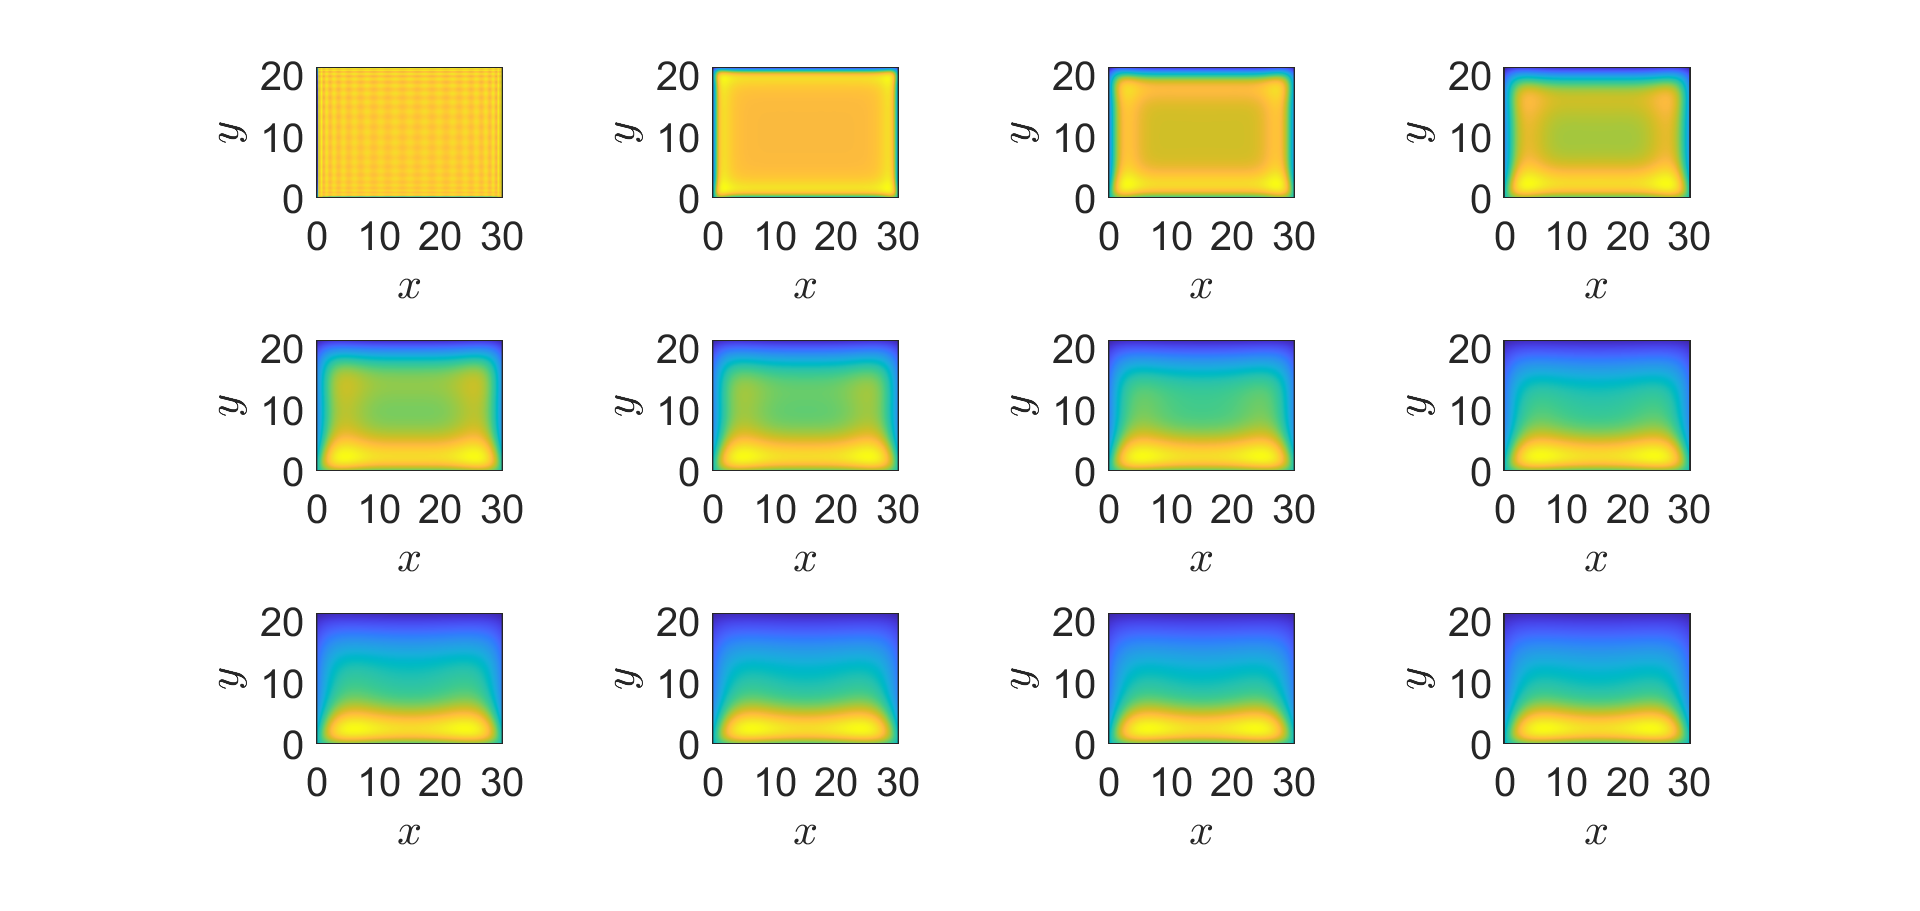
\includegraphics[scale=0.35]{Ex8F1b.png}
%	\caption{Figure 8 Example, $\bar \rho = 0.036$, $\sigma = 1$, $12$ different times} 
%	\label{F1b}
%\end{figure}
%If I instead decrease $\bar \rho$  to $0.036$, the sediment is more spread out at the bottom.
%
%I then change the initial condition to be non-symmetric: $\bar \rho = 0.072 (1 + \cos(\pi / 30 y_1)\cos(\pi / 30 y_2))$. This has the effect that the final distribution is asymmetric as well, see Figure \ref{Fx}. This is done with $N = 40$, which is again not quite enough for numerical stability, but it takes $1$ min $20$ seconds to solve.
%\begin{figure}[h]
%	\centering
%	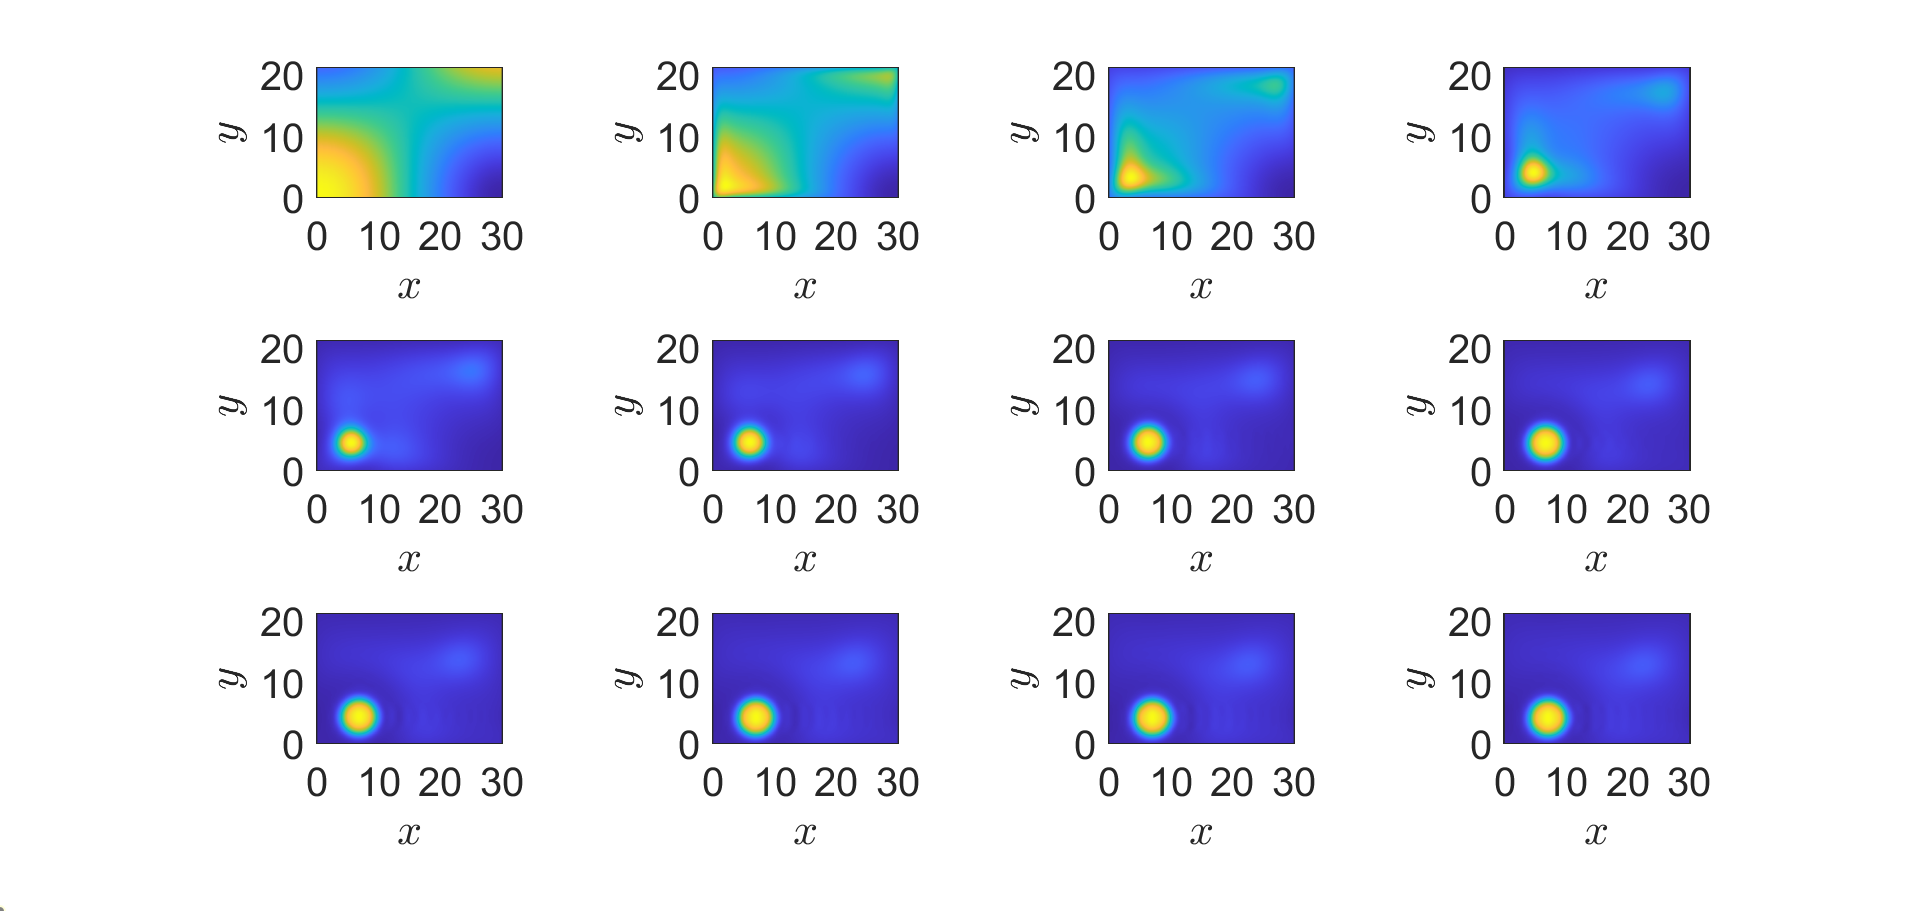
\includegraphics[scale=0.4]{Ex8NonSym.png}
%	\caption{Figure 8 Example, $\bar \rho = 0.072$, $\sigma = 1$, $12$ different times, asymmetric initial condition} 
%	\label{Fx}
%\end{figure}
%\subsubsection{Example Figure 10}
%In this example everything stays the same except that more density is in the system, $\bar \rho \sigma^2 = 0.2$. We start with $\sigma = 1$ and $\bar \rho = 0.2$, which needs more points for numerical stability. We try $N = 50$. This is still not quite enough but better and takes $8$ minutes to solve, see Figure \ref{F4}. We can see the sort of behaviour that is visible in the paper, that the different clusters merge. I think if we let time run longer it'd merge into one.
%\begin{figure}[h]
%	\centering
%	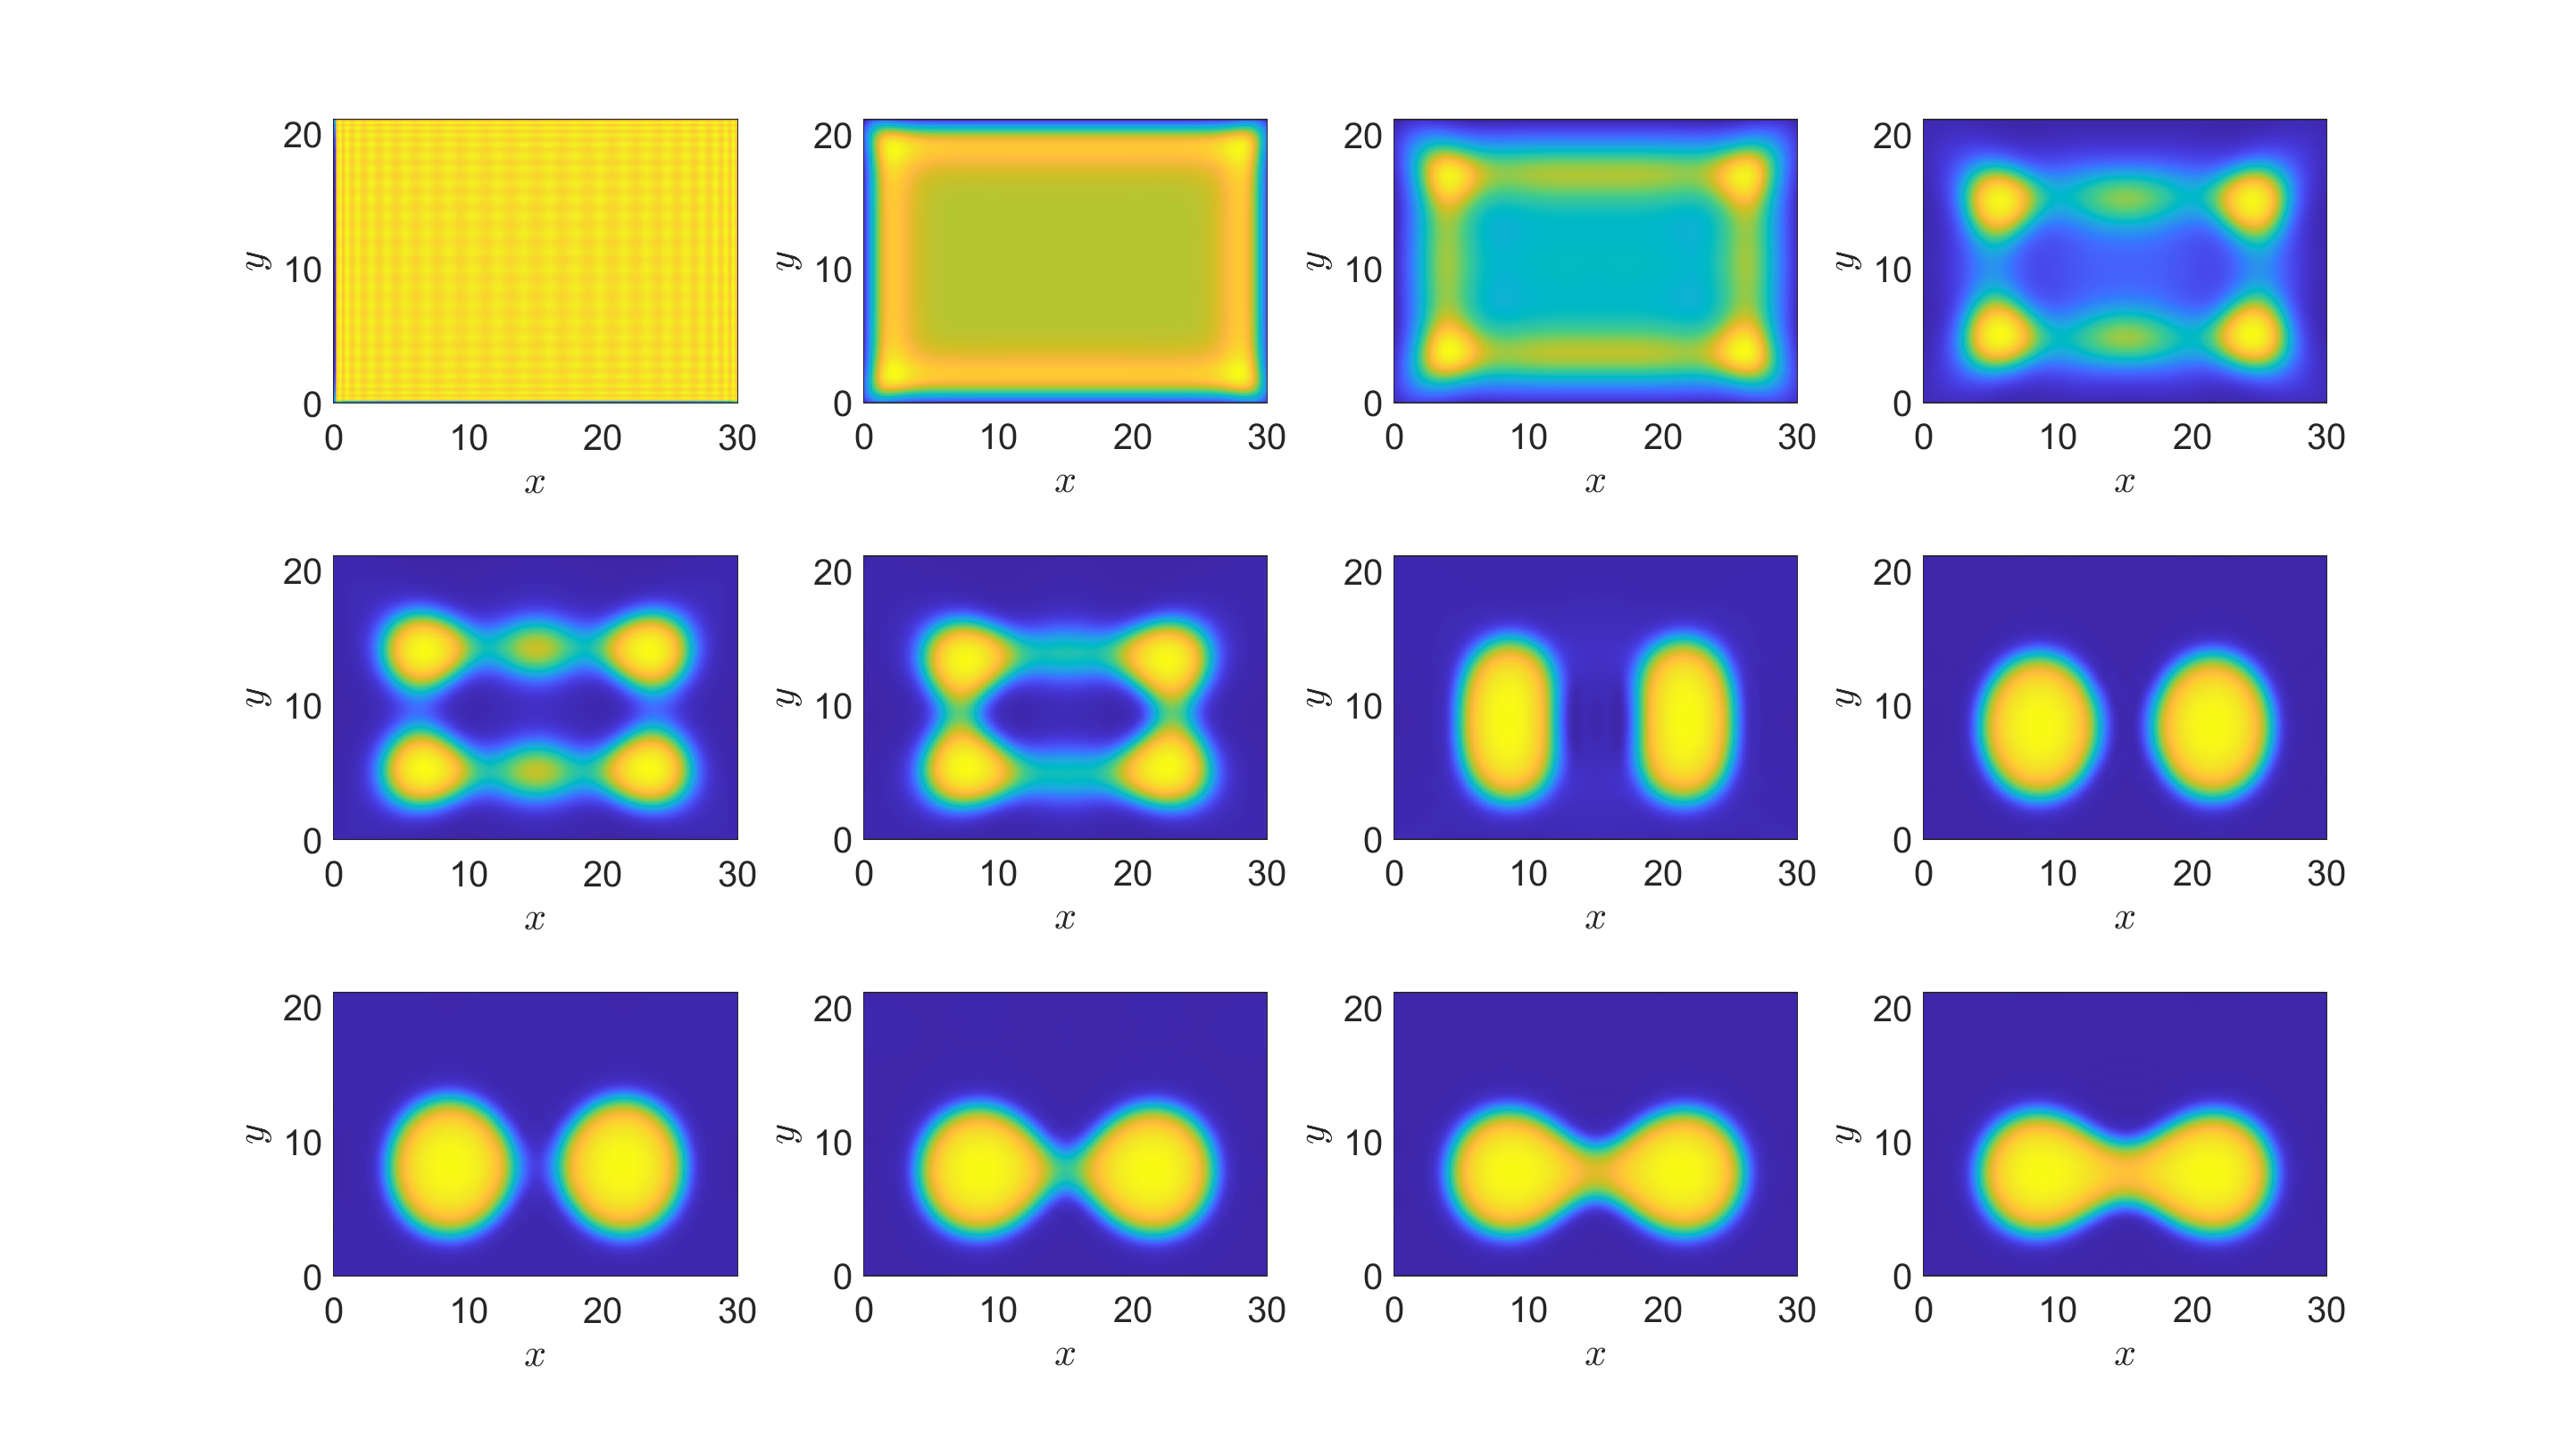
\includegraphics[scale=0.25]{Ex10F1.png}
%	\caption{Figure 10 Example, $\bar \rho = 0.2$, $\sigma = 1$, $12$ different times} 
%	\label{F4}
%\end{figure} 
%Again, since we have half of the original domain, we set $\sigma = 0.6$. We use $60$ points but that is not enough again as can be seen in Figure \ref{F4a}.
%\begin{figure}[h]
%	\centering
%	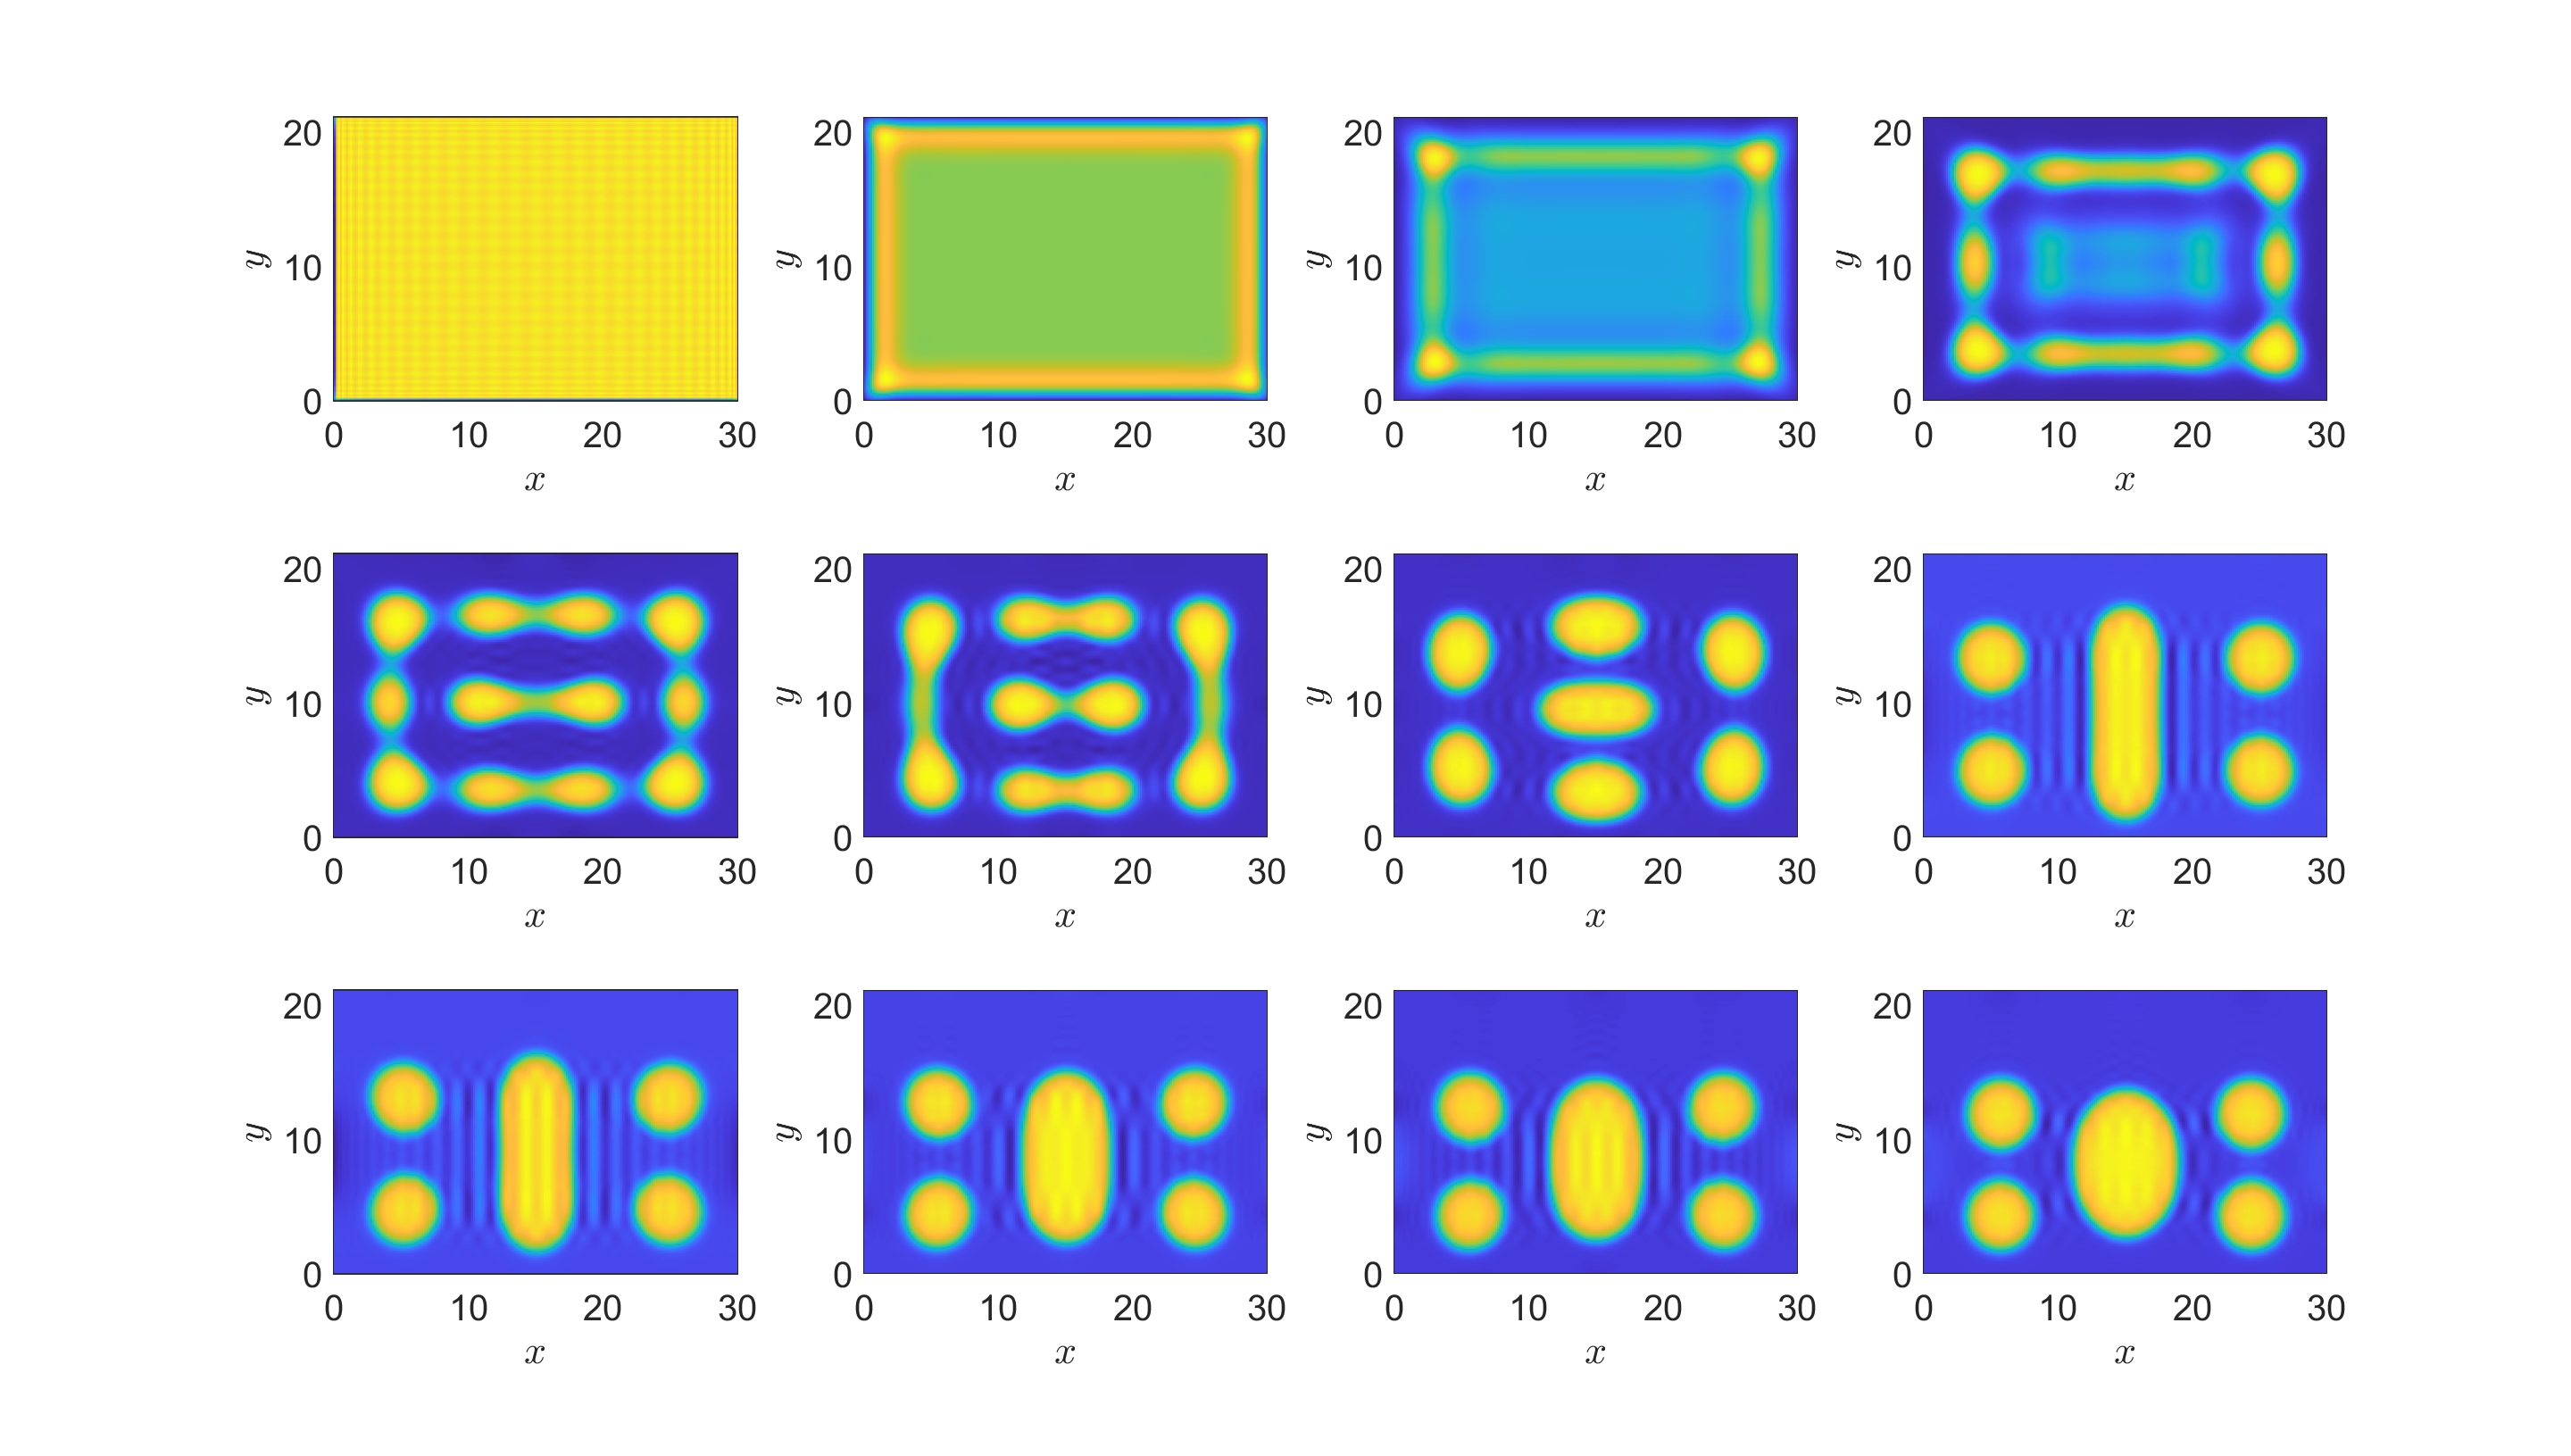
\includegraphics[scale=0.25]{Ex10F2.png}
%	\caption{Figure 10 Example, $\bar \rho = 0.2$, $\sigma = 0.6$, $12$ different times} 
%	\label{F4a}
%\end{figure} 

\subsection{Replicating examples from the paper in a periodic box}
%Since the original simulations are done in a periodic box, we implement the problem in the periodic box as well. We expect near identical results to the paper, given that the setup is now identical.
%We choose a periodic box that has no flux boundary conditions on the top and bottom of the box, while being periodic on the sides. 
%We scale time as done in Equation \eqref{Eq1}, so that the time scales are comparable. In order to get qualitatively good results, we choose $n =100$ and $N = 100$. This takes approximately five hours to solve. In Figures \ref{F5} and \ref{F6} the results for the configurations corresponding to Figure 8 in Archer's paper can be seen ($ \bar \rho = 0.072$, choosing $\sigma = 1$, and running up to $T = 300$). In Figures \ref{F7} and \ref{F8} we see the results that correspond to the configurations in Figure 10 in Archer's paper ($ \bar \rho = 0.2$, choosing $\sigma = 1$, running time up to $T = 300$). While the results for Archer's first result look very close to the original, the second set of results is a little different. This may have to do with slightly different initial conditions or numerical solutions.
%
%
%\begin{figure}[h]
%	\centering
%	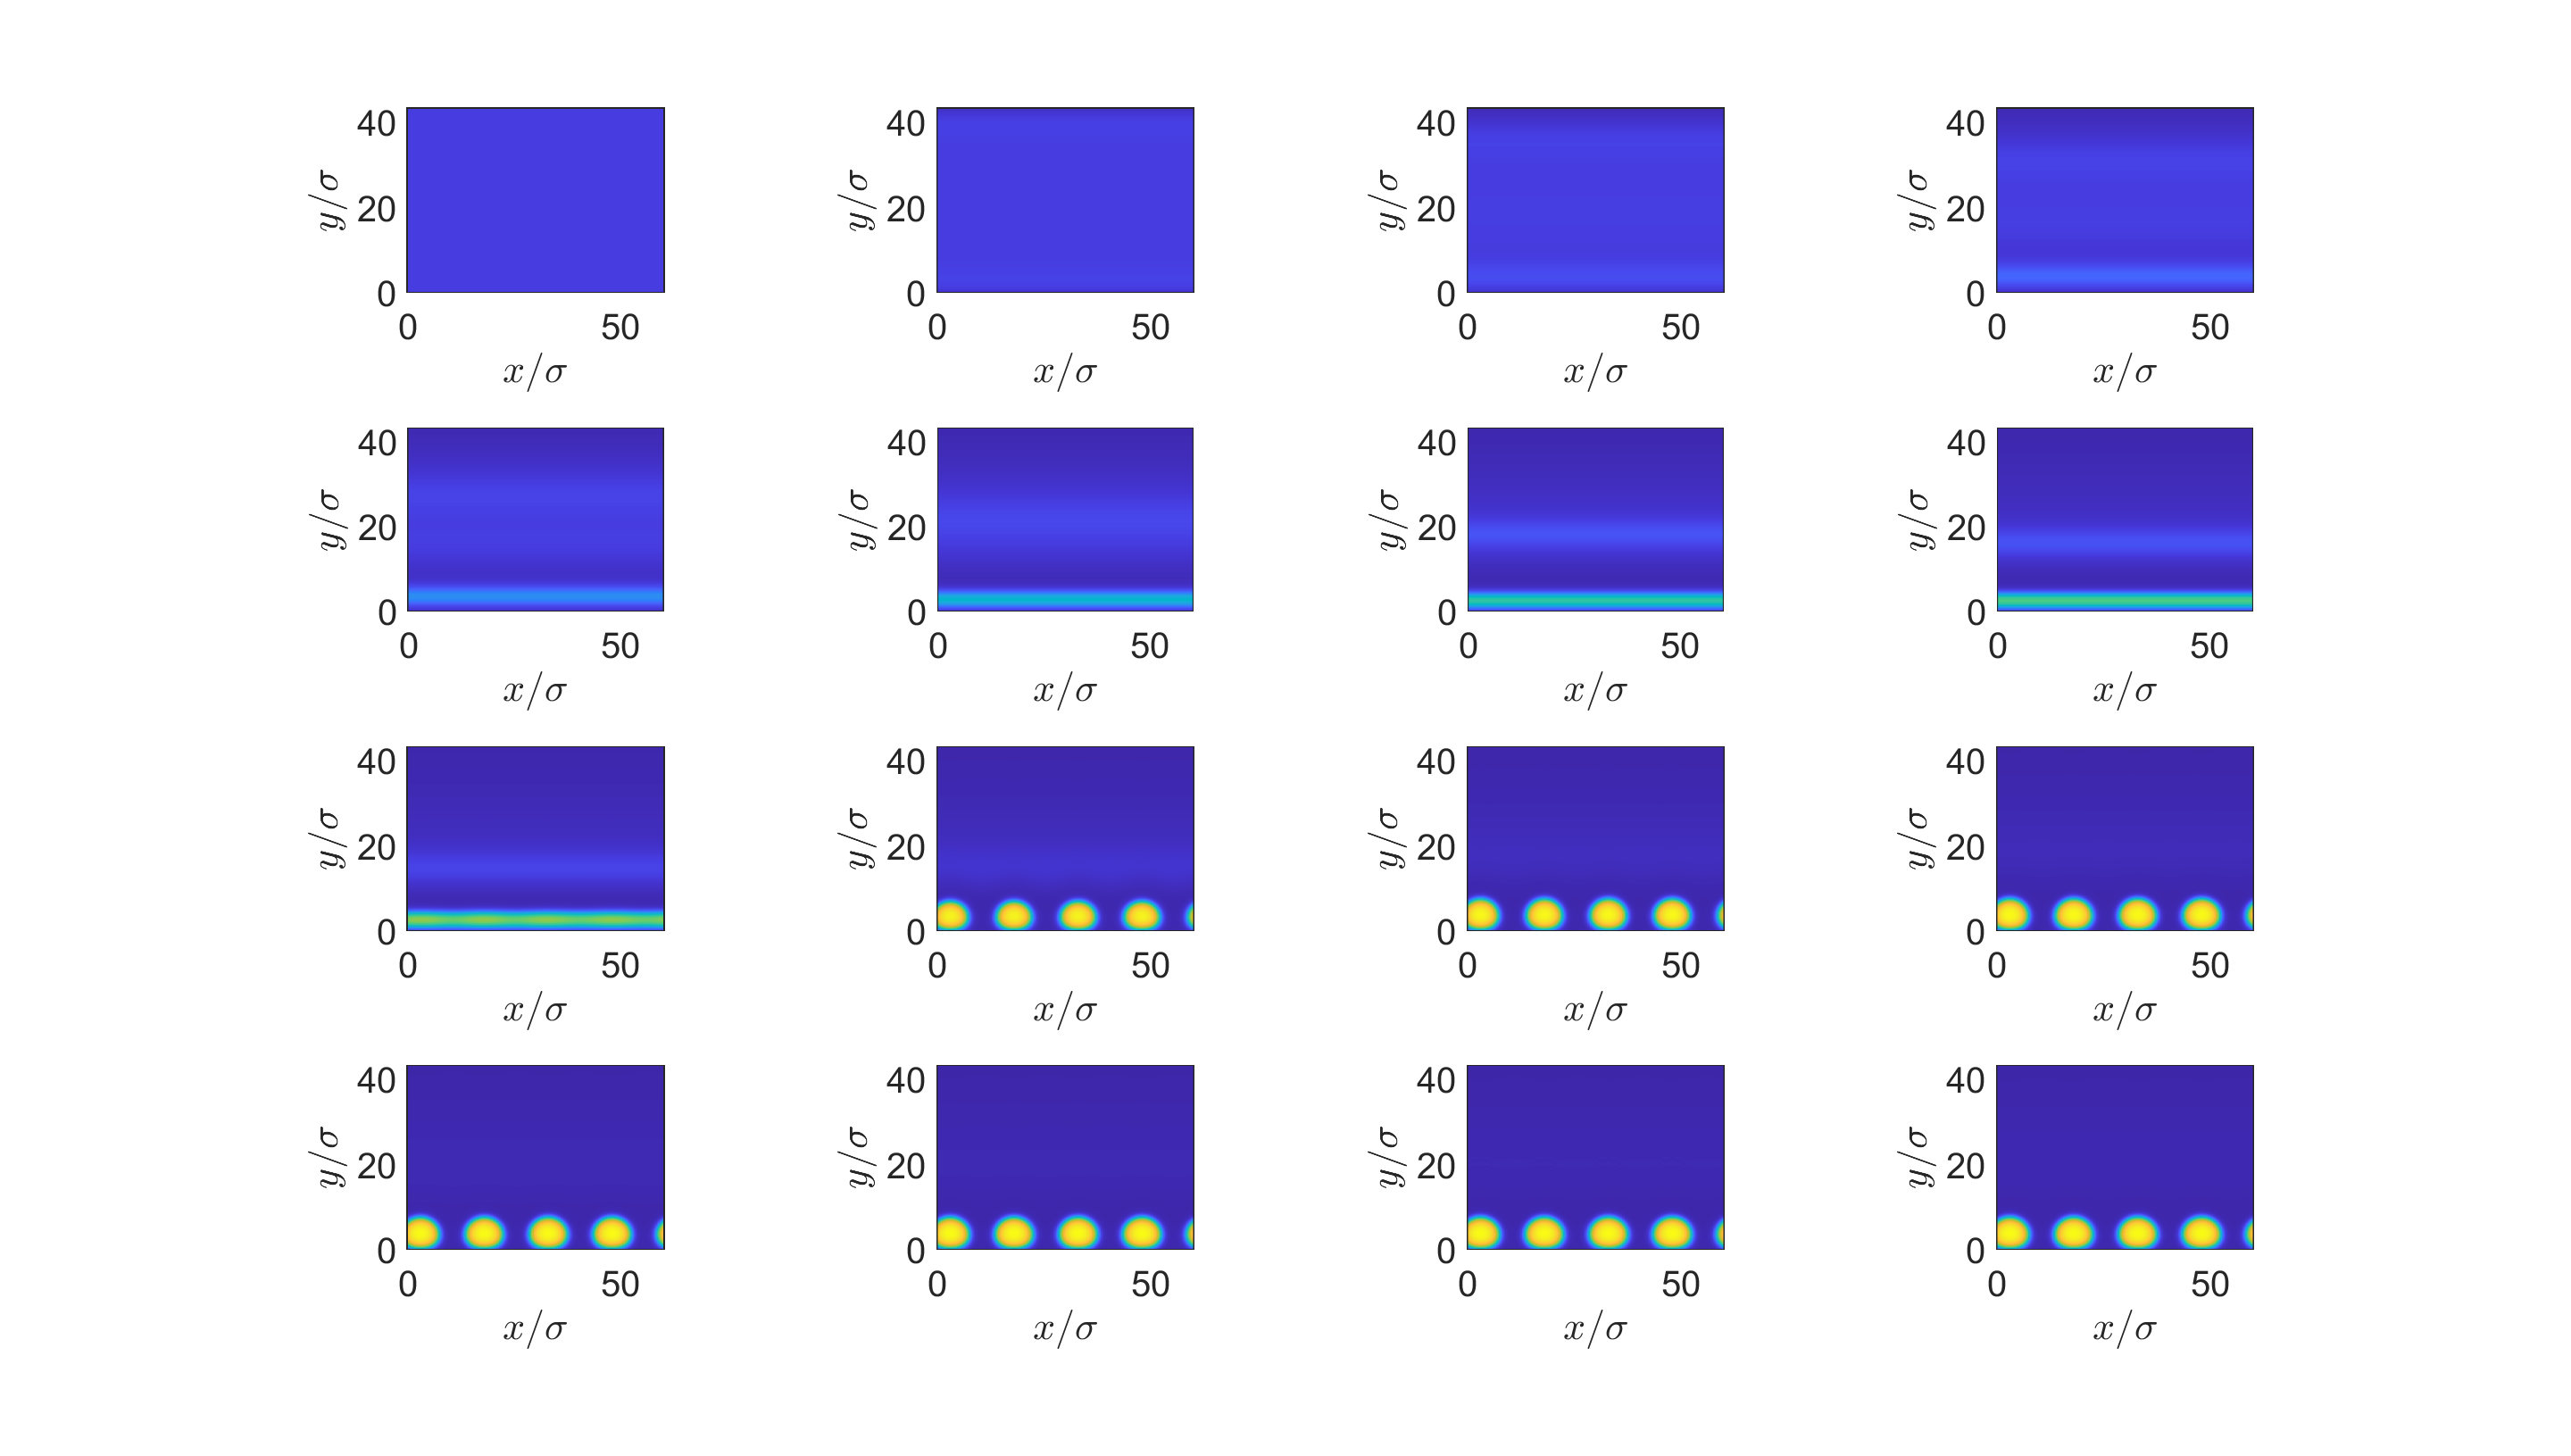
\includegraphics[scale=0.25]{Plotrhobar0072.png}
%	\caption{Figure 8 in paper, result at each time} 
%	\label{F5}
%\end{figure}
%\begin{figure}[h]
%	\centering
%	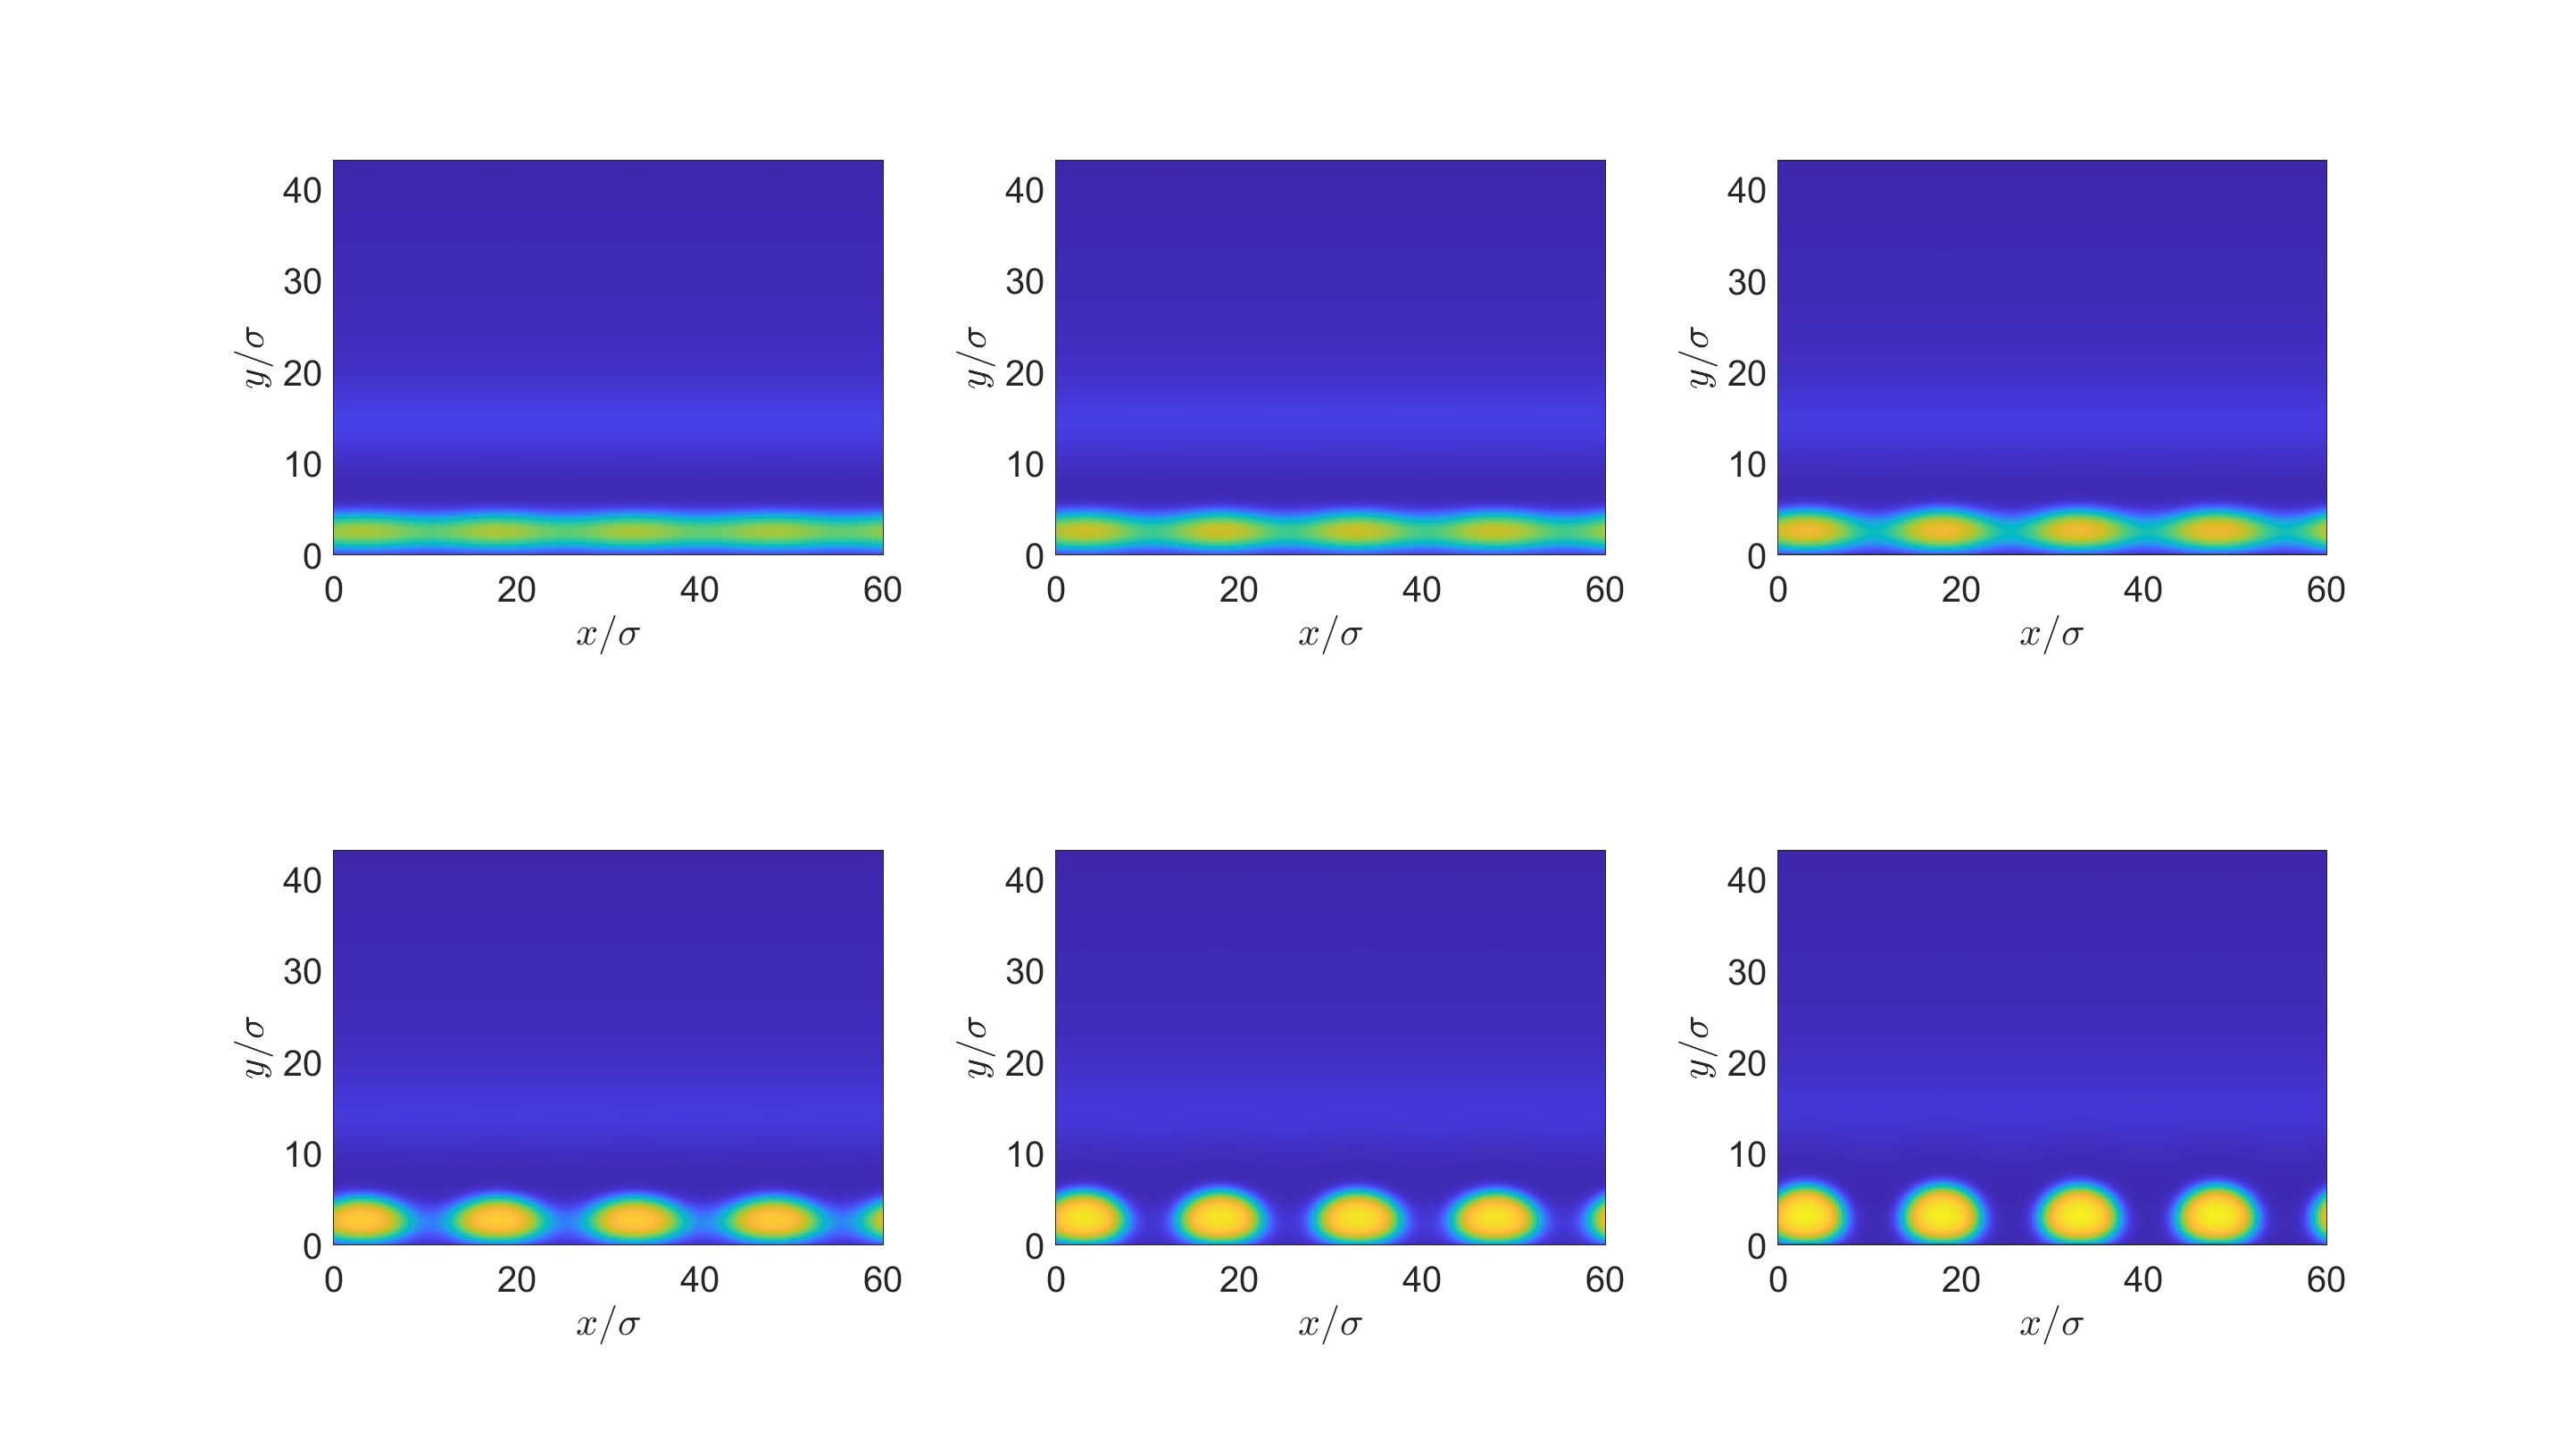
\includegraphics[scale=0.25]{rhobar0072Zoom57to62.png}
%	\caption{Figure 8 in paper, result at times 57 - 62 out of 100} 
%	\label{F6}
%\end{figure}
%
%\begin{figure}[h]
%	\centering
%	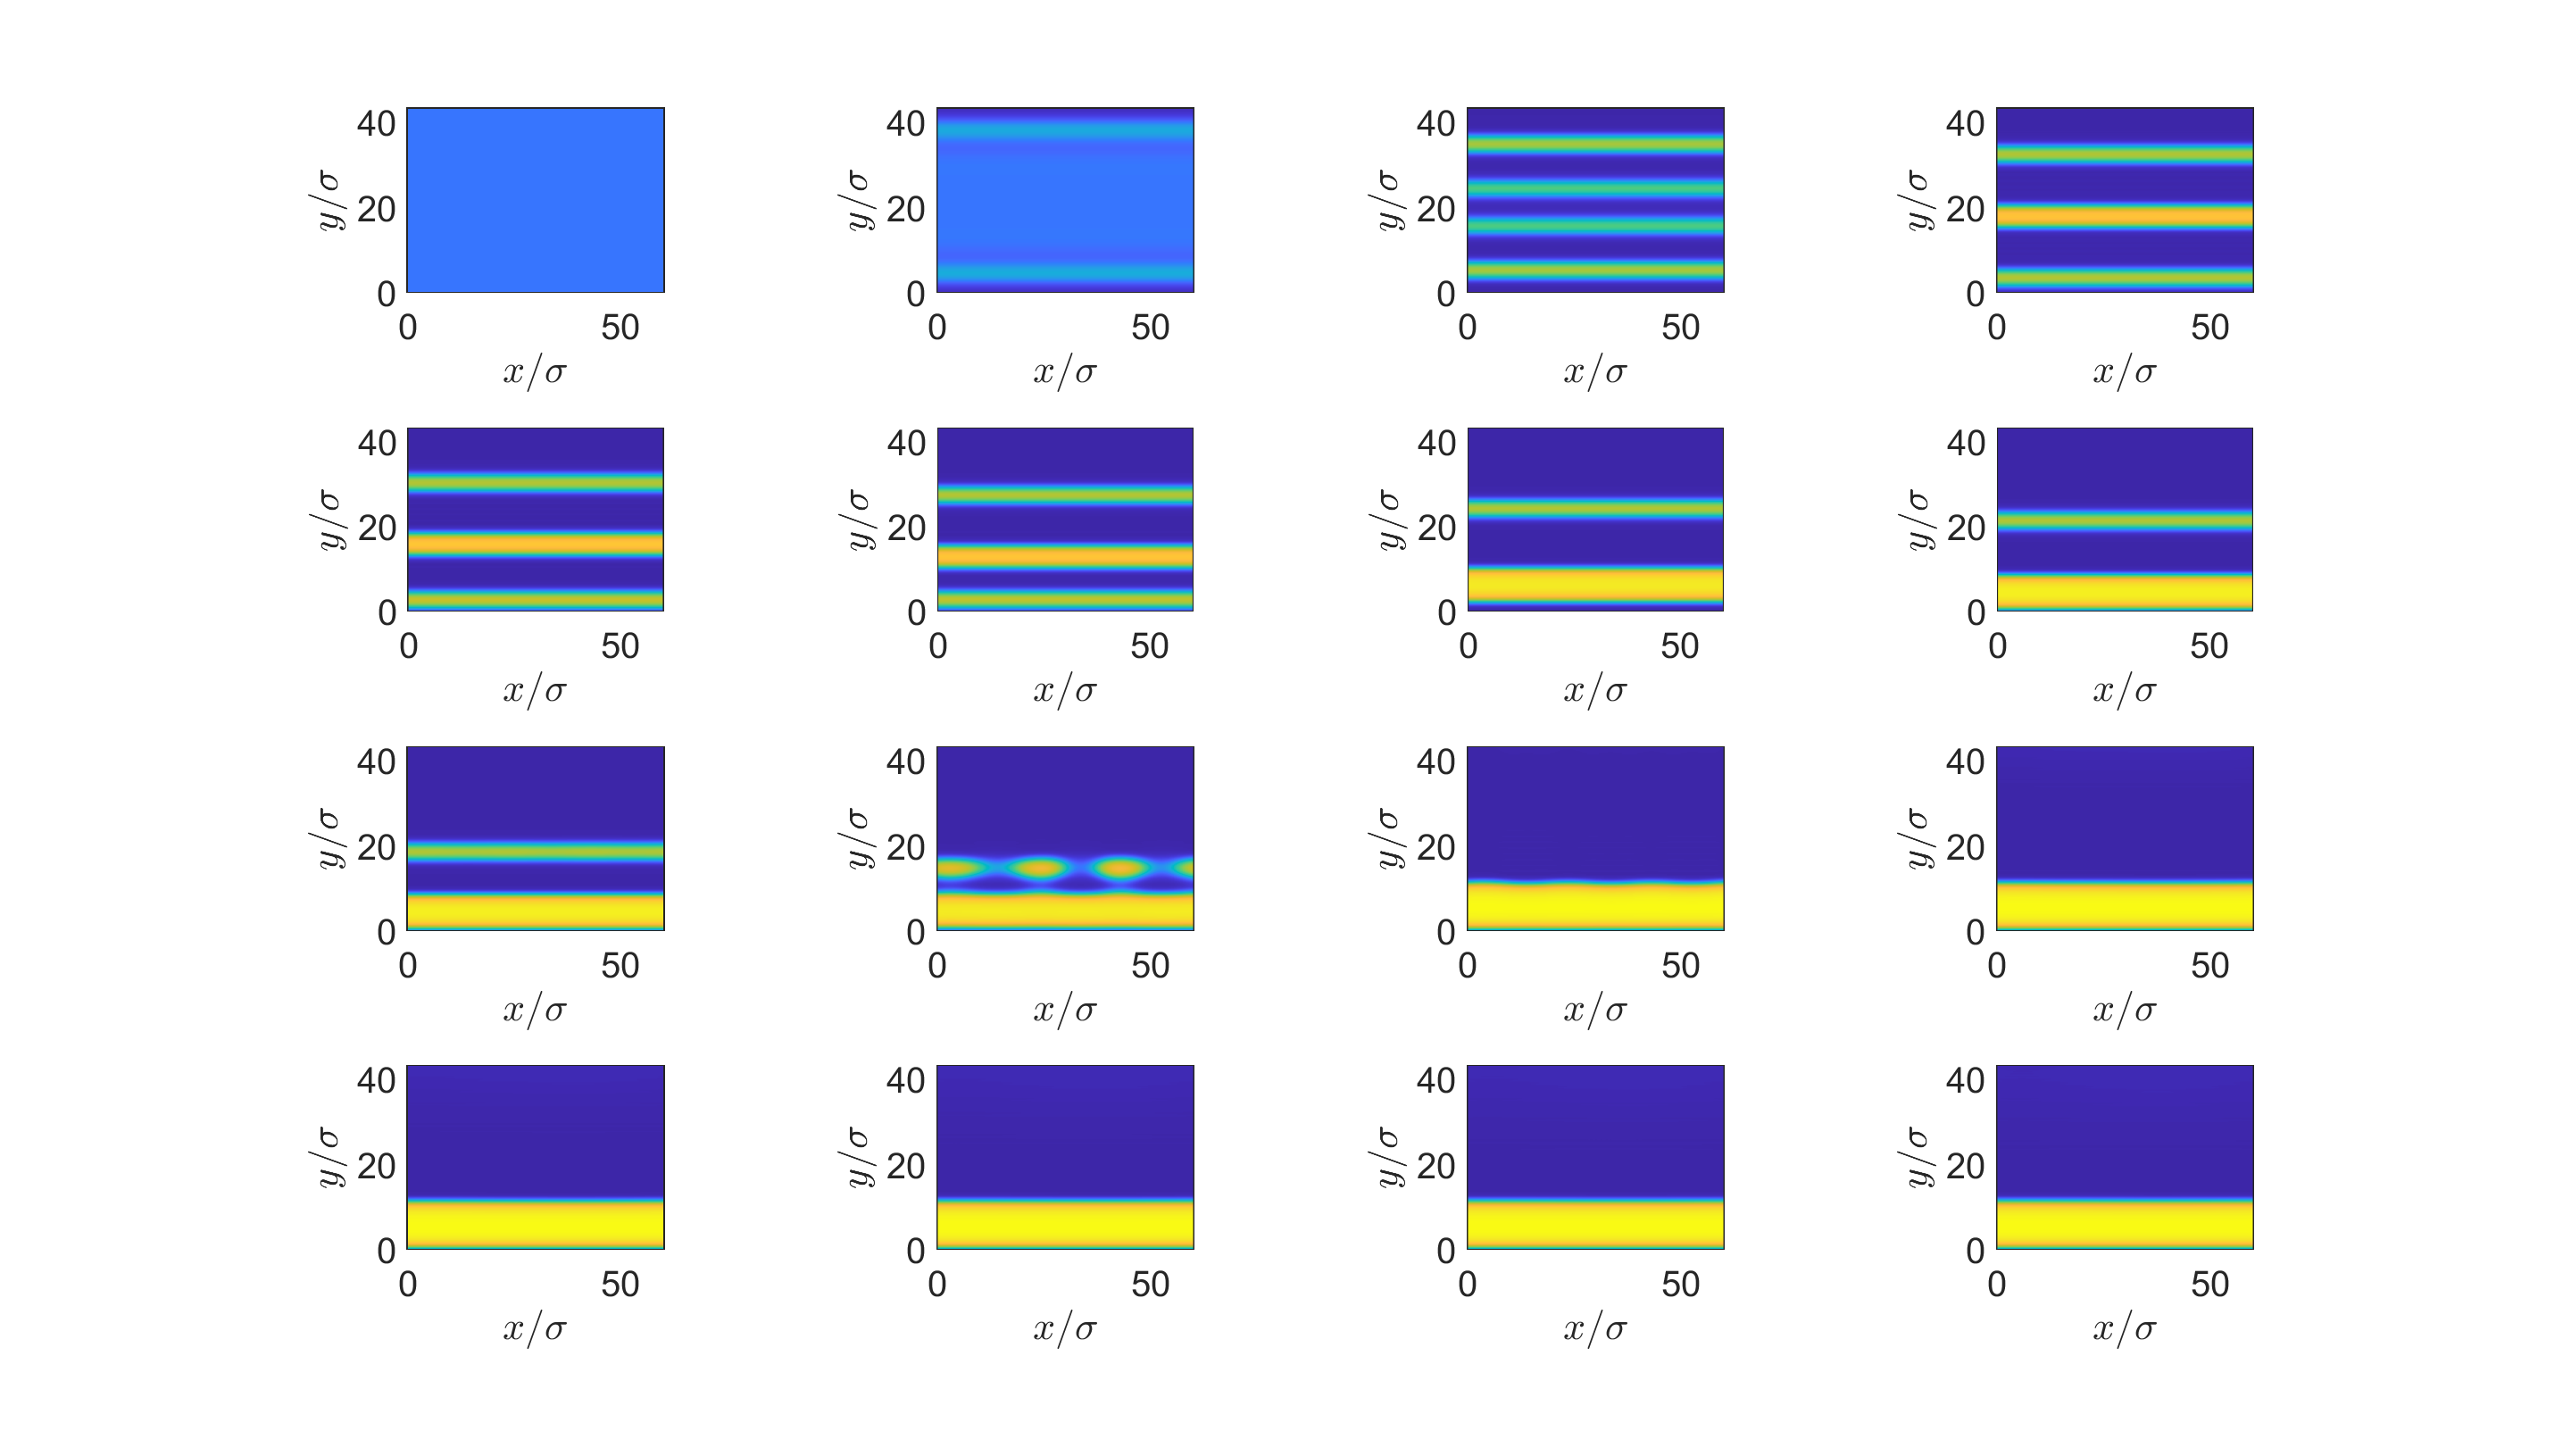
\includegraphics[scale=0.25]{Plotrhobar02.png}
%	\caption{Figure 10 in paper, result at each time} 
%	\label{F7}
%\end{figure}
%\begin{figure}[h]
%	\centering
%	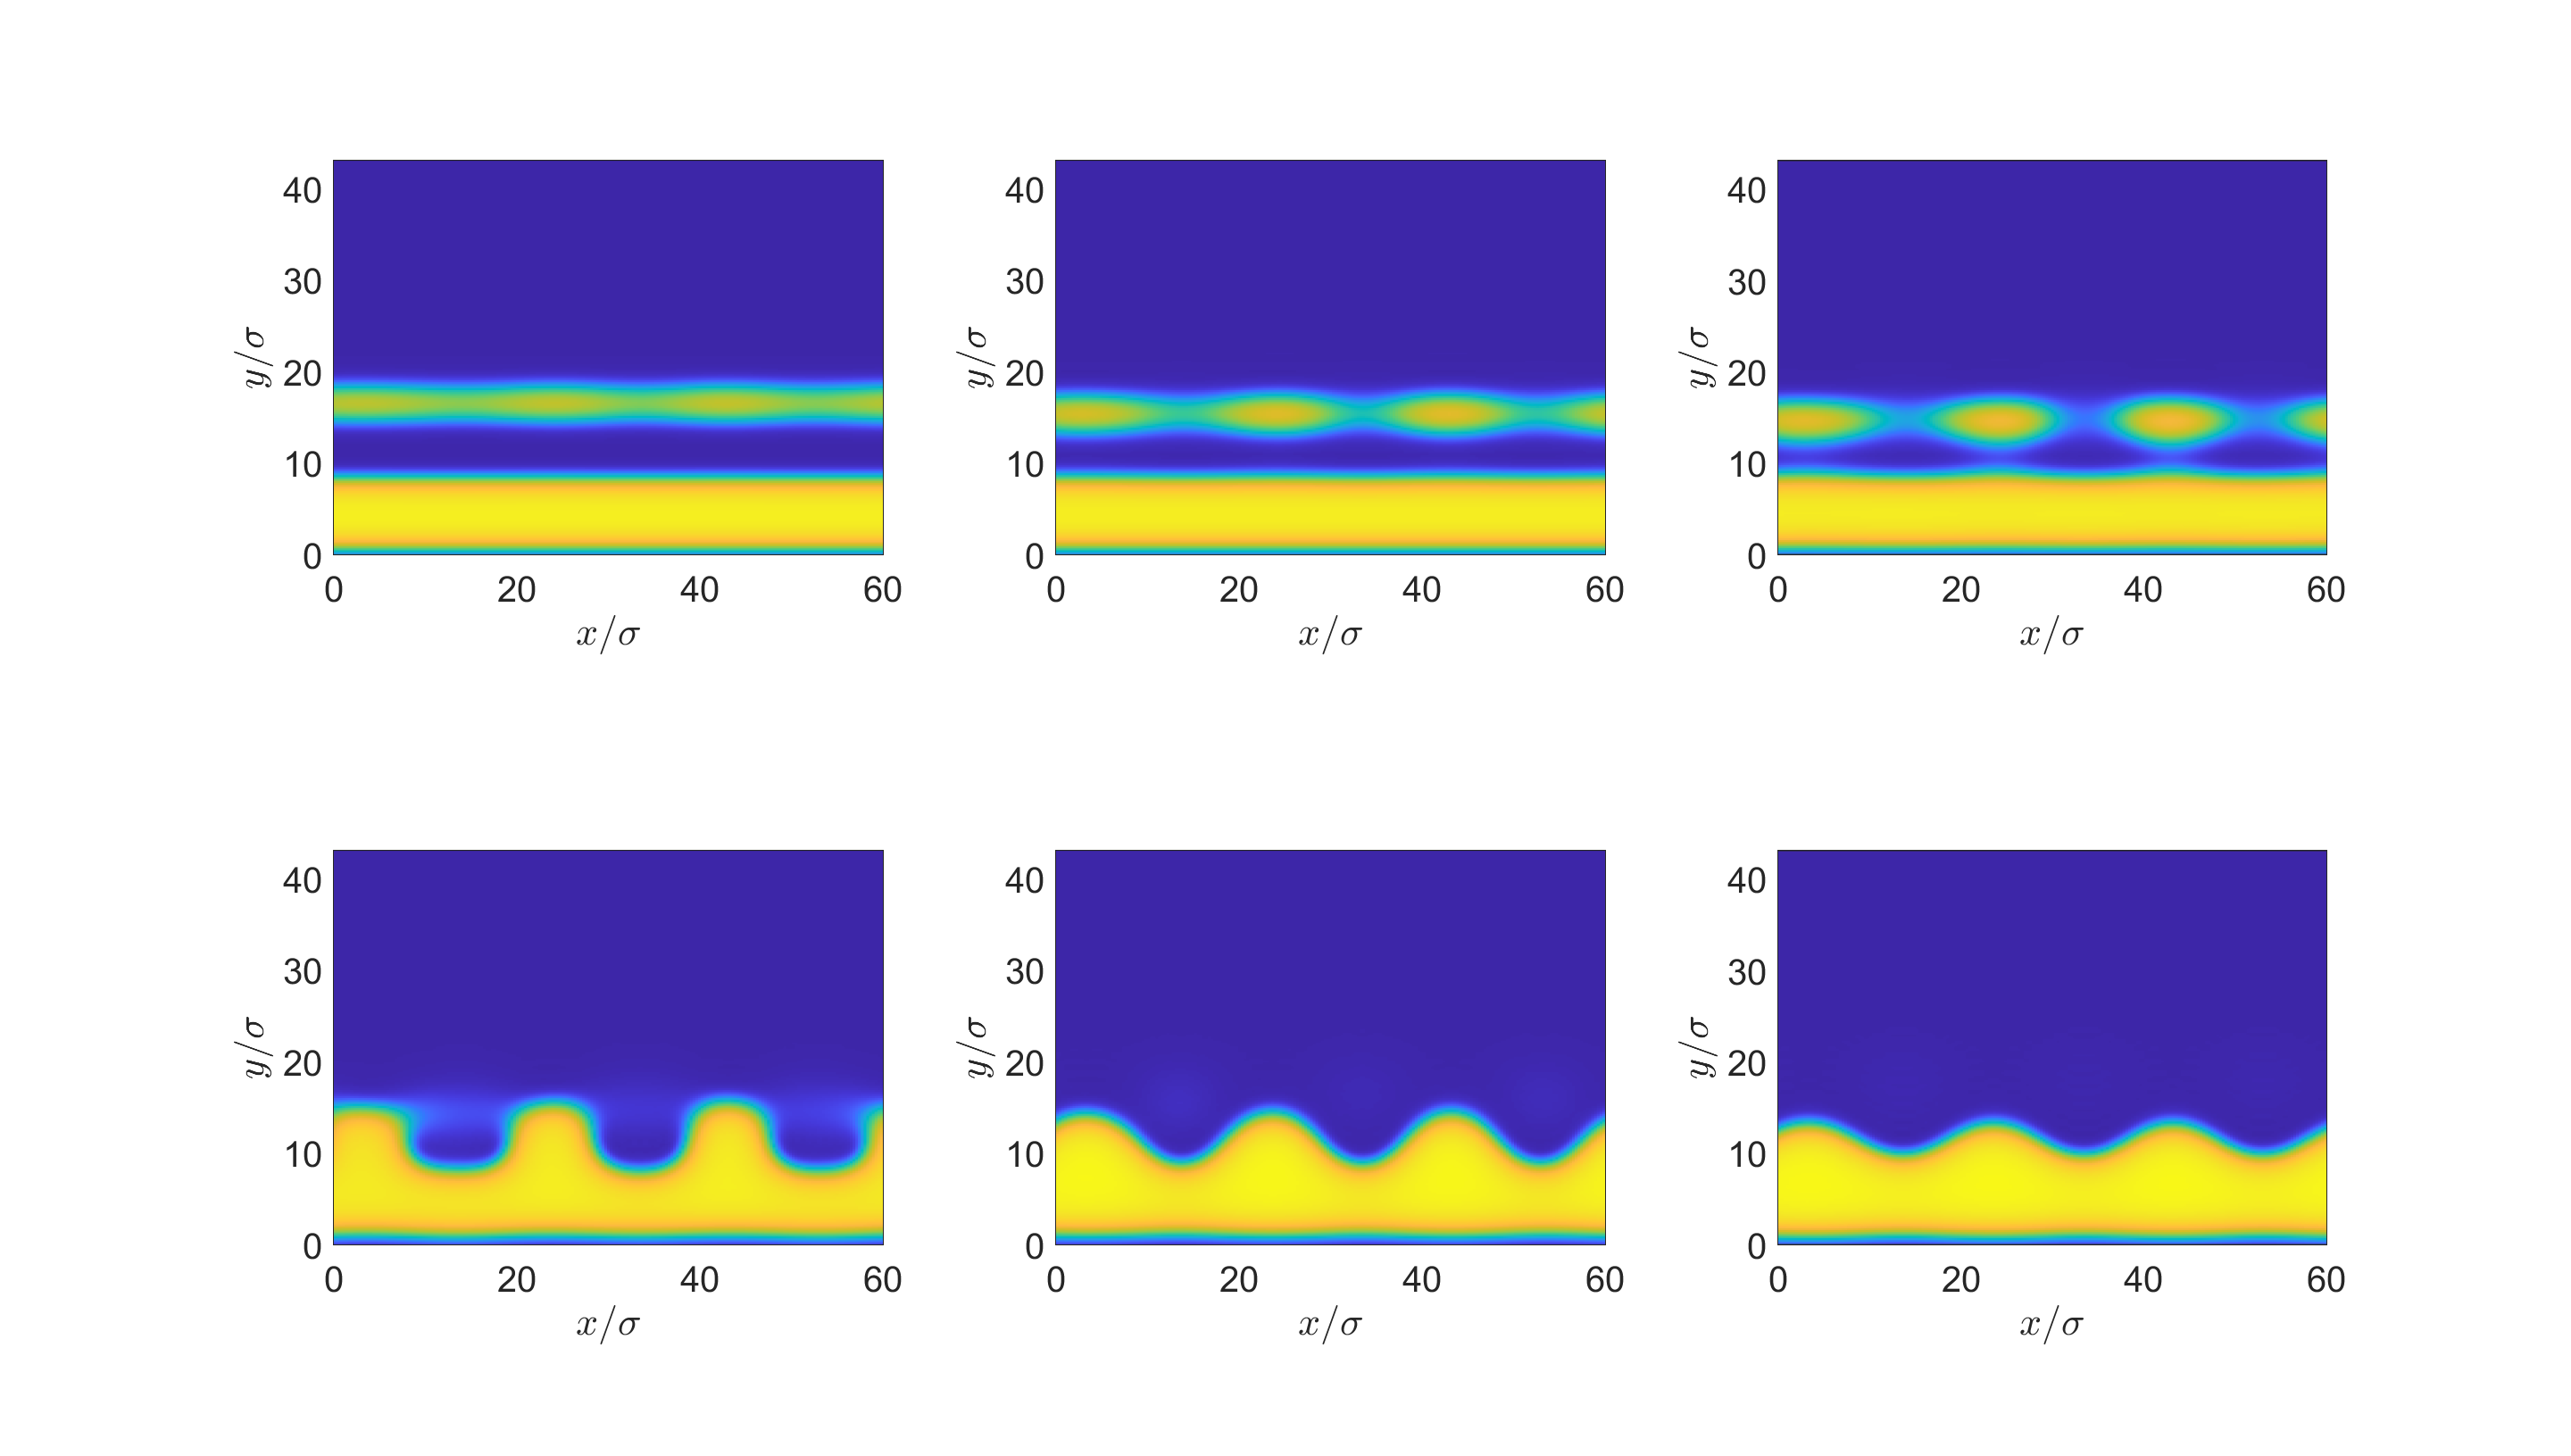
\includegraphics[scale=0.25]{rhobar02Zoom60to66.png}
%	\caption{Figure 8 in paper, result at times 60 - 66 out of 100} 
%	\label{F8}
%\end{figure}
%
%
%


\subsection{Optimization Problems}
\subsubsection{Optimization in a Box}
%We have $N = 40$ and $n = 30$. We choose the ODE tolerance to be $10^{-7}$ and the optimization tolerance is $10^{-3}$.
%I fixed the problems with the implementation of the sedimentation optimization code. First, I tested whether setting $\hr = \rho_{FW}$ would converge within one iteration. This happened. 
%Then I set up a test problem which sets $\hr$ to be the forward solution for $V_{ext} = ay$, where $a = 0.1$, as in Archer's paper. Then I set up the optimization forward problem to be such that $a = 0.01$ and $\w = \mathbf 0$. We expect the control to act downward, since the strength of gravity $a$ is decreased.
%We also expect that the cost $\mathcal J$ is decreasing from the baseline $J_{FW}$ when optimizing.
%For $\beta = 10^{-3}$ and $\beta = 10^{-1}$ this works well.
%When $\beta = 10^{-3}$ we get $J_{FW} = 0.4955$ and $J_{Opt} = 0.0556 $. 
%The results can be seen in Figures \ref{Fa1}, \ref{Fa2} and \ref{Fa3}.
%\begin{figure}[h]
%	\centering
%	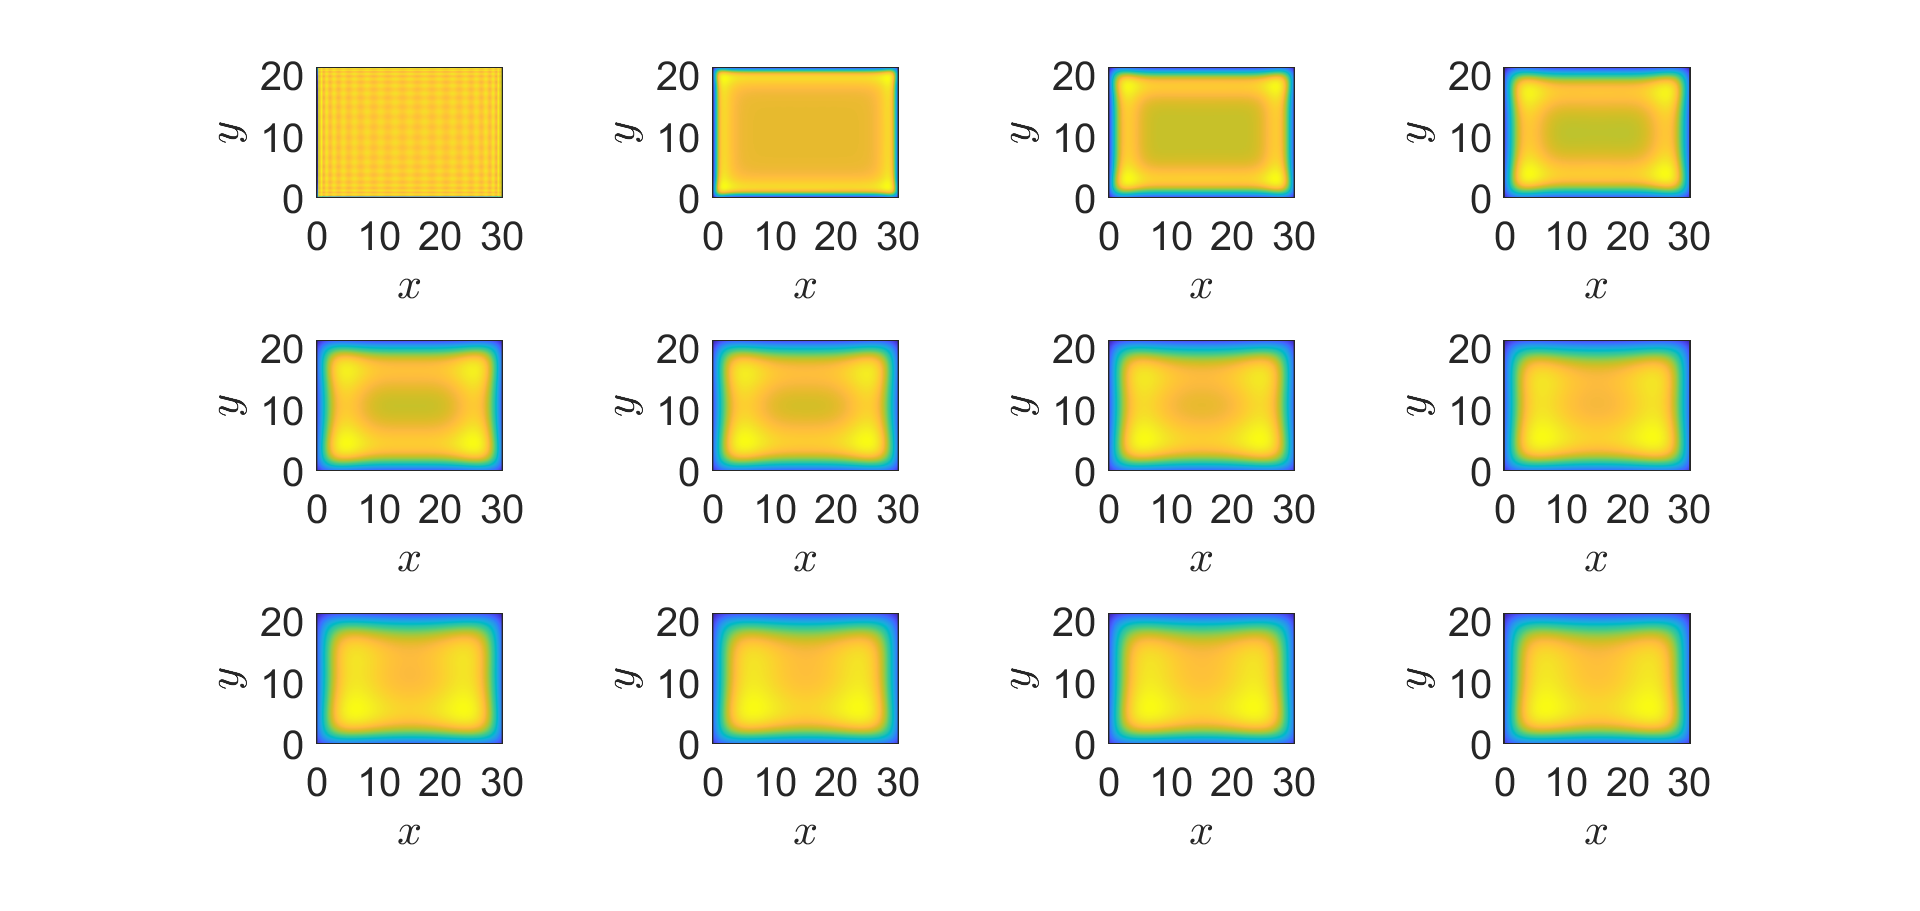
\includegraphics[scale=0.35]{F11.png}
%	\caption{Forward $\rho$ for $a = 0.01$} 
%	\label{Fa1}
%\end{figure}	
%\begin{figure}[h]
%	\centering
%	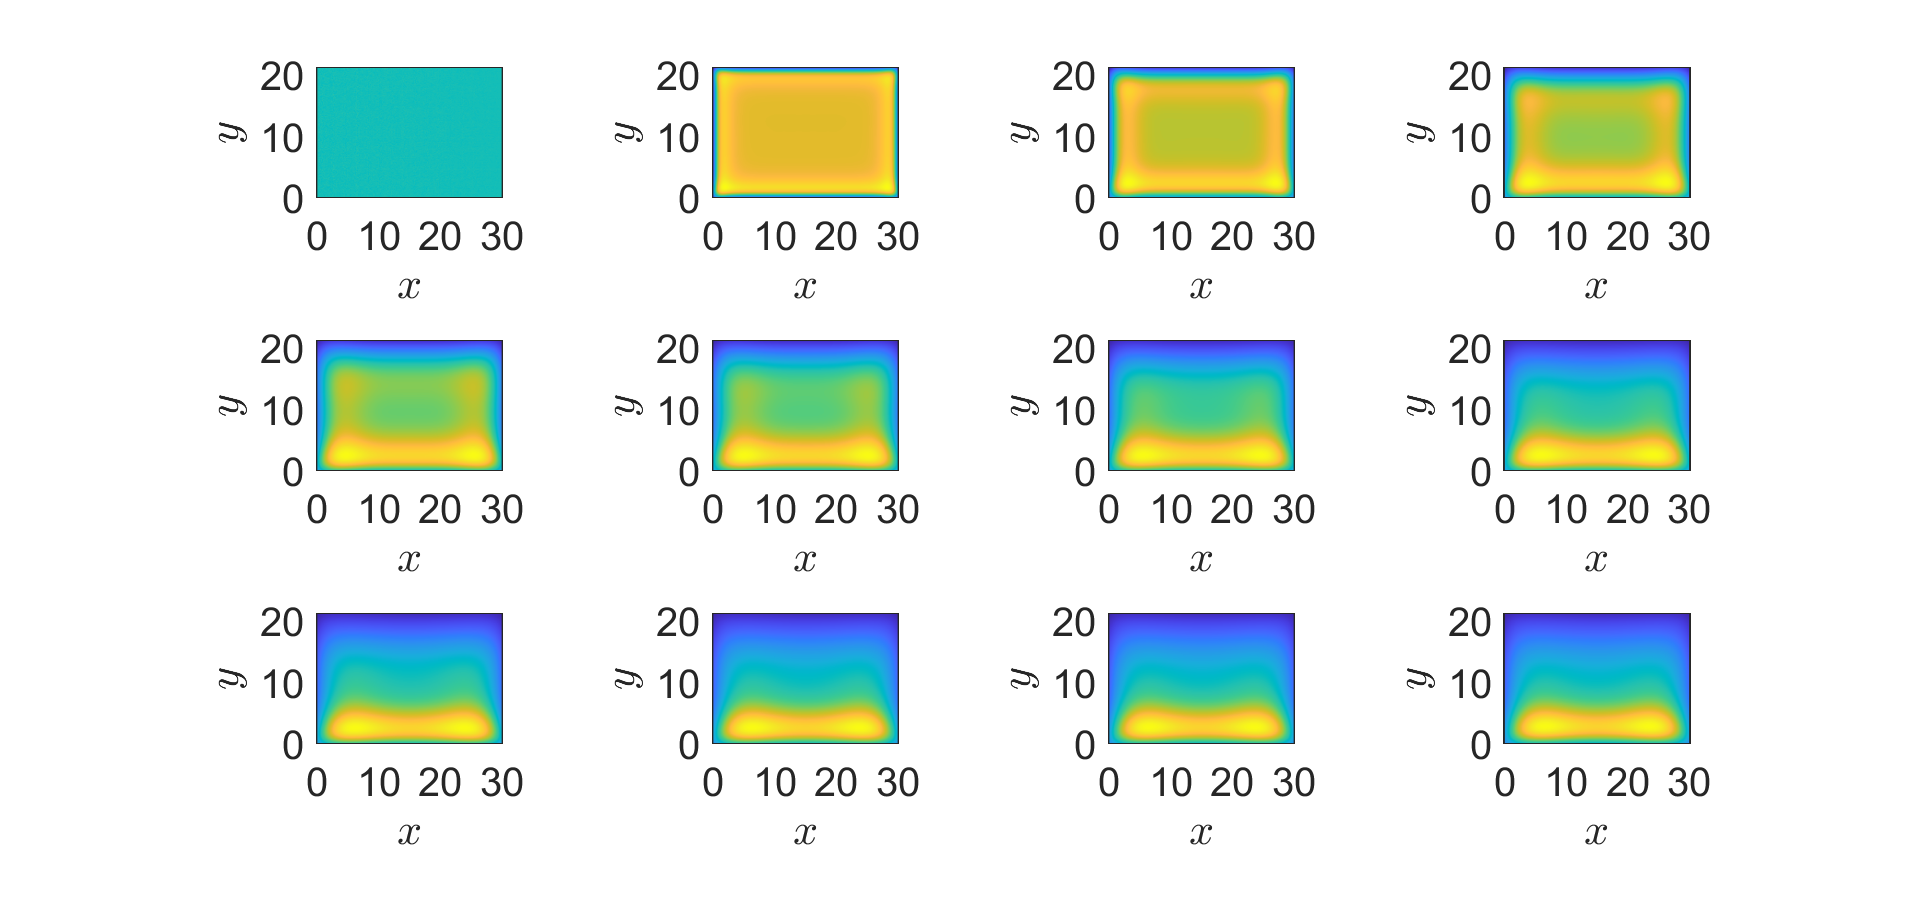
\includegraphics[scale=0.35]{F21.png}
%	\caption{Optimal $\rho$ for $a = 0.01$} 
%	\label{Fa2}
%\end{figure}
%\begin{figure}[h]
%	\centering
%	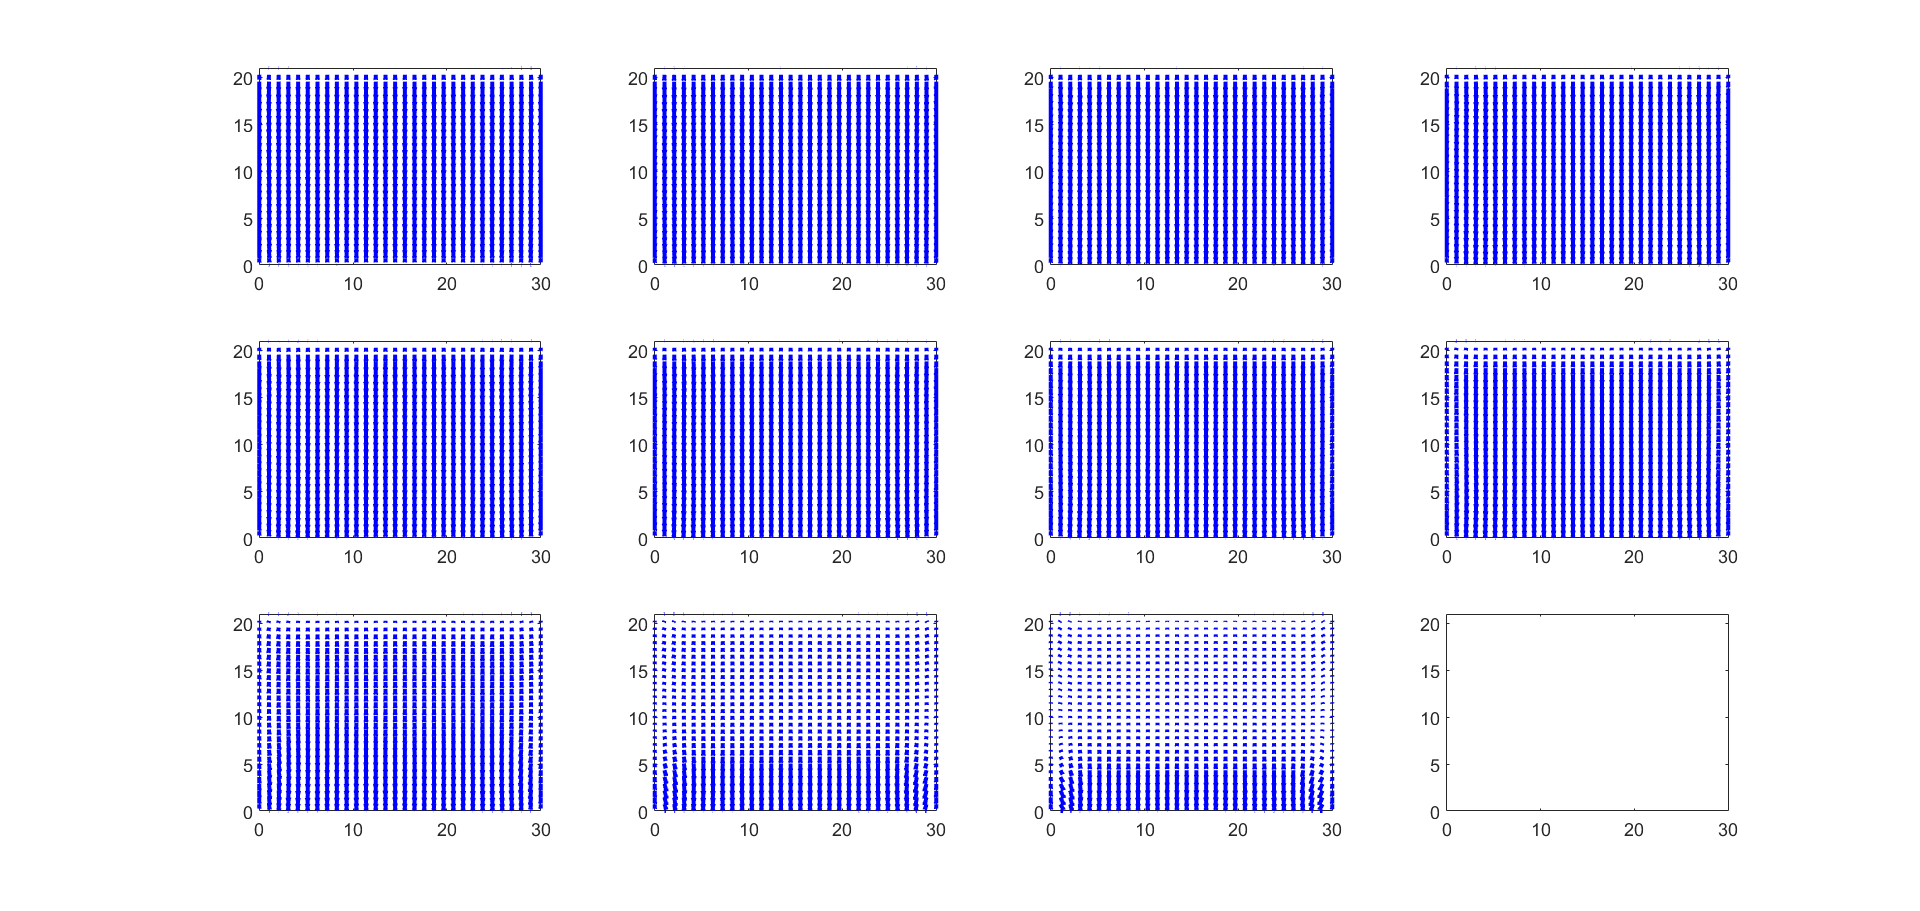
\includegraphics[scale=0.35]{F31.png}
%	\caption{Optimal Control for $a = 0.01$} 
%	\label{Fa3}
%\end{figure}
%
%

\subsubsection{Optimization in a Box - Time-Independent Control}
%This result can be used for other forward problems as well, since only the terms involving the control are affected here. Therefore, we apply the result to the sedimentation equations.
%We have $N = 40$ and $n = 30$ for each shape. We choose the ODE tolerance to be $10^{-7}$ and the optimization tolerance is $10^{-3}$.
%I set up a test problem which sets $\hr$ to be the forward solution for $V_{ext} = ay$, where $a = 0.1$, as in Archer's paper. Then I set up the optimization forward problem to be such that $a = 0.01$ and $\w = \mathbf 0$. We expect the control to act downward, since the strength of gravity $a$ is decreased.
%We also expect that the cost $\mathcal J$ is decreasing from the baseline $J_{FW}$ when optimizing.
%The gradient equation is:
%\begin{align*}
%	\w = - \frac{1}{\beta}\int_0^T \rho \nabla q dt.
%\end{align*}
%This means, we get a $\w$ which is averaged over the time horizon and therefore time independent. This seems to work well. $J_{FW} = 0.4855$ and $J_{Opt} = 0.0733$. The results can be seen in Figures \ref{F6a}, \ref{F7a} and \ref{F8a}.
%
%\begin{figure}[h]
%	\centering
%	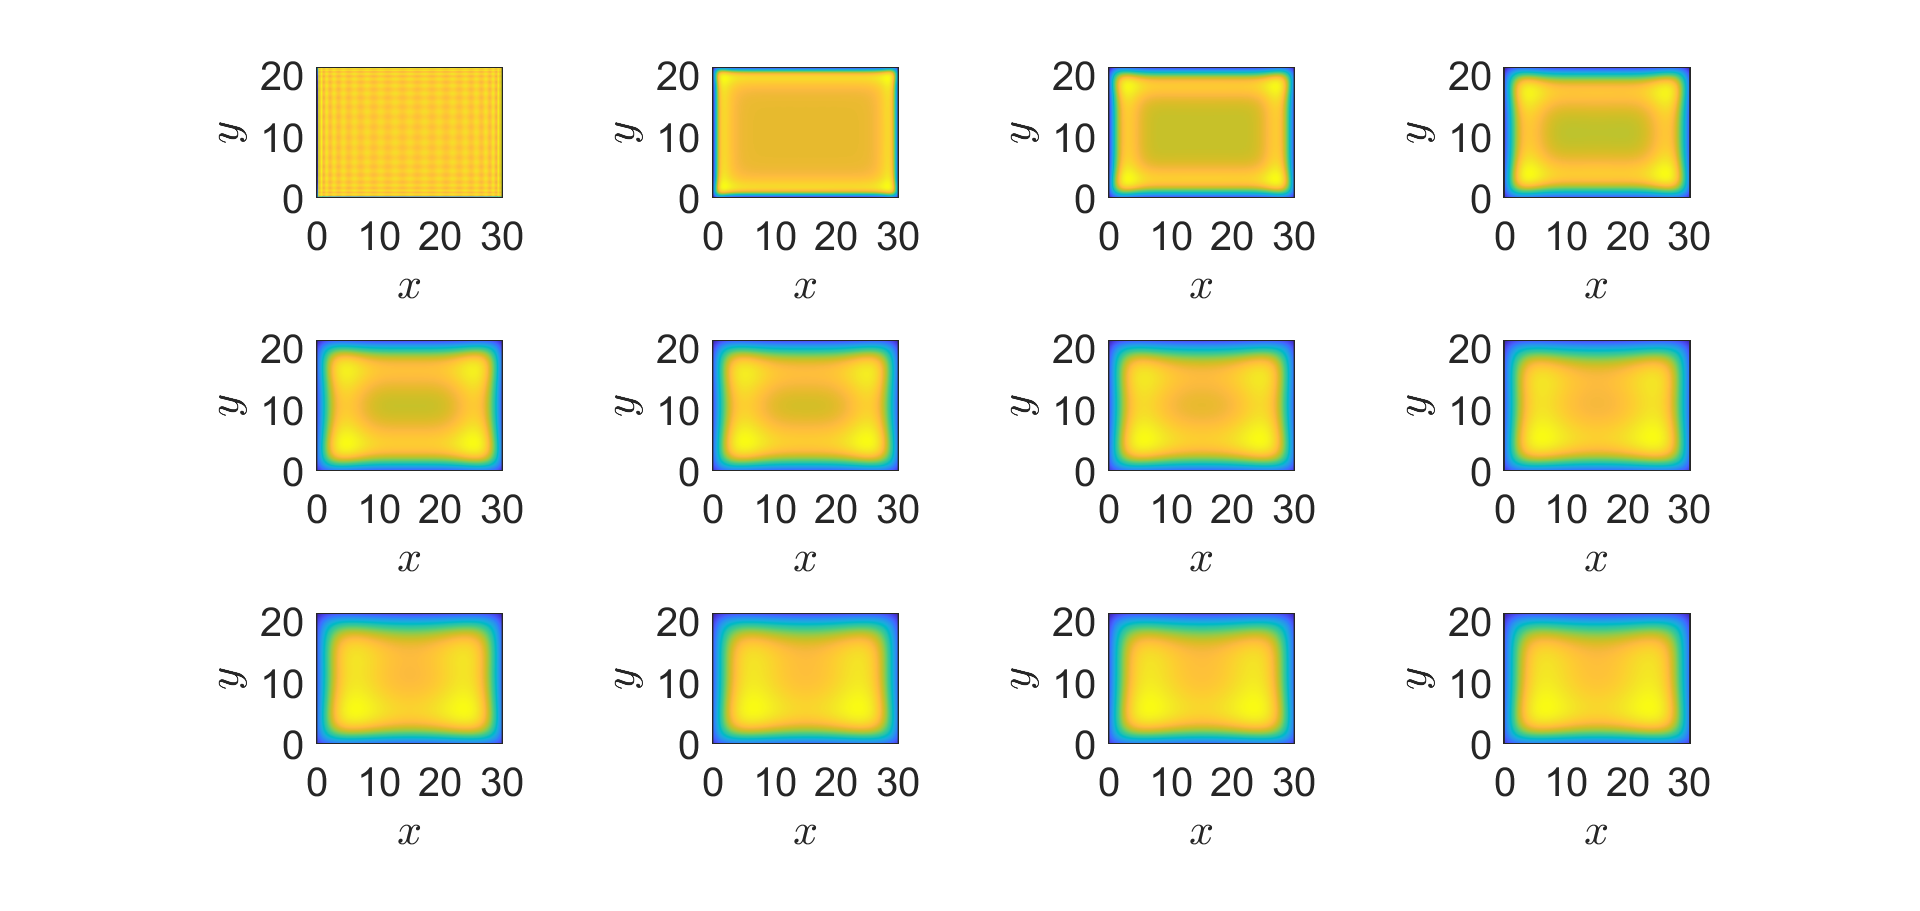
\includegraphics[scale=0.35]{C1.png}
%	\caption{Time-independent; Forward $\rho$ for $a = 0.01$} 
%	\label{F6a}
%\end{figure}	
%\begin{figure}[h]
%	\centering
%	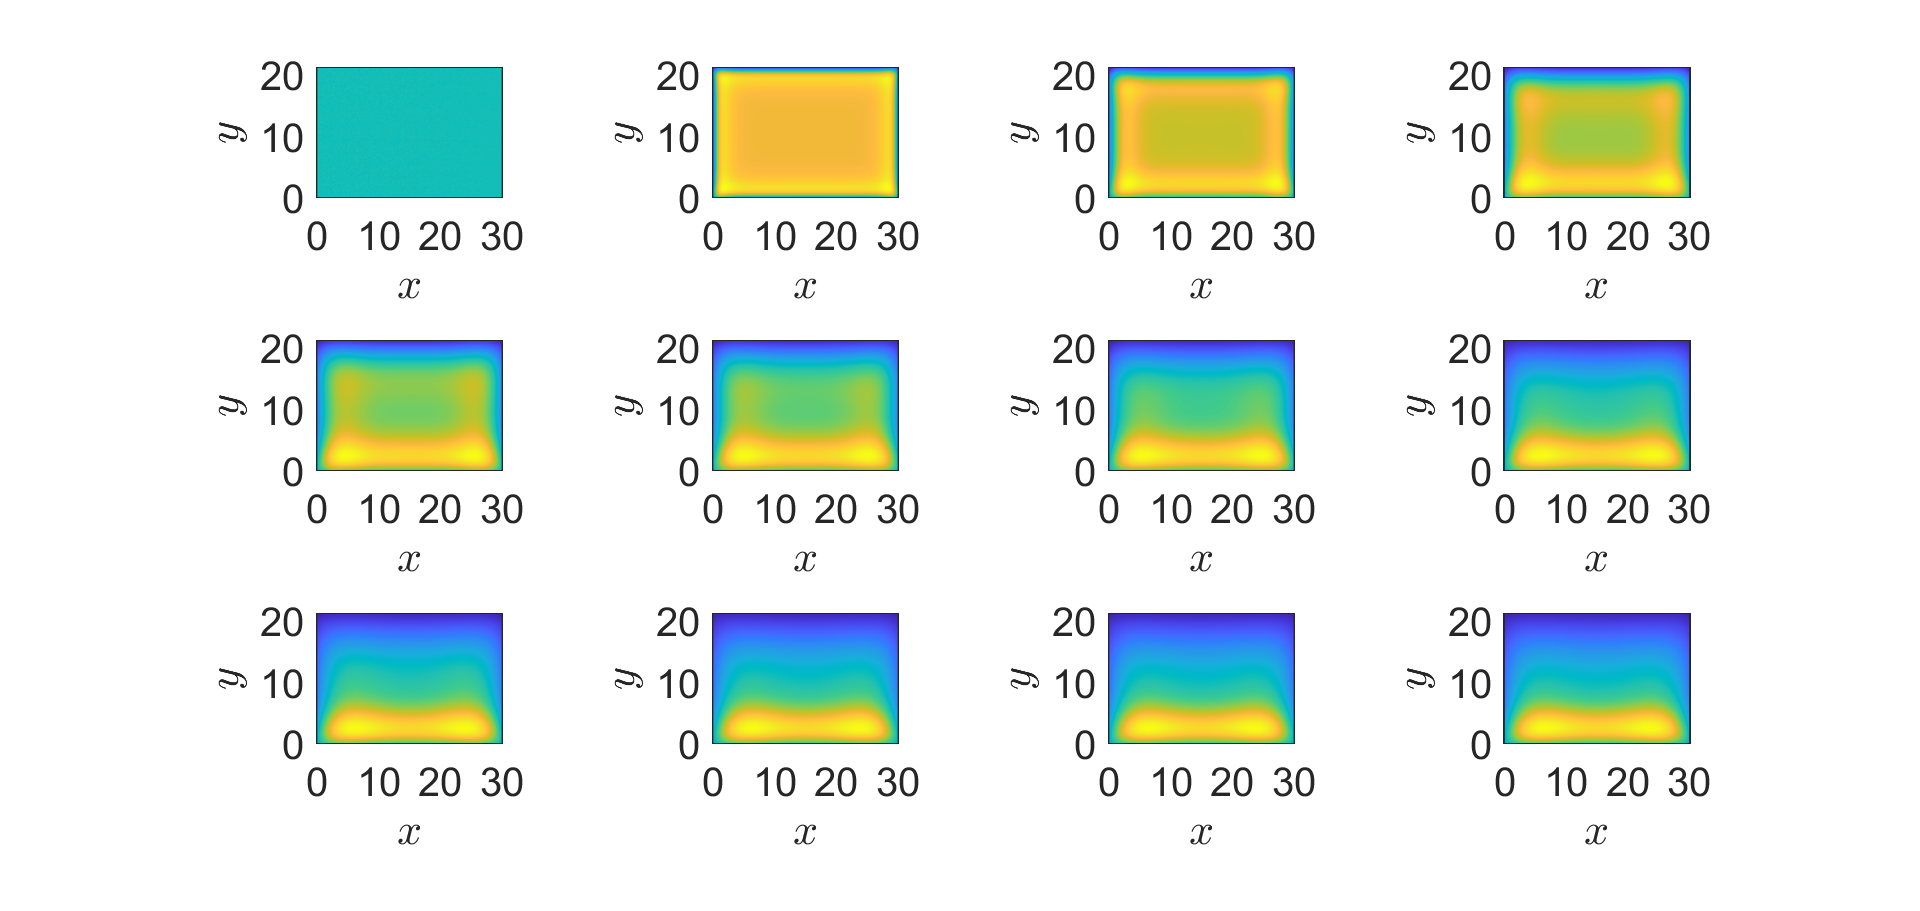
\includegraphics[scale=0.35]{C2.png}
%	\caption{Time-independent; Optimal $\rho$ for $a = 0.01$} 
%	\label{F7a}
%\end{figure}
%\begin{figure}[h]
%	\centering
%	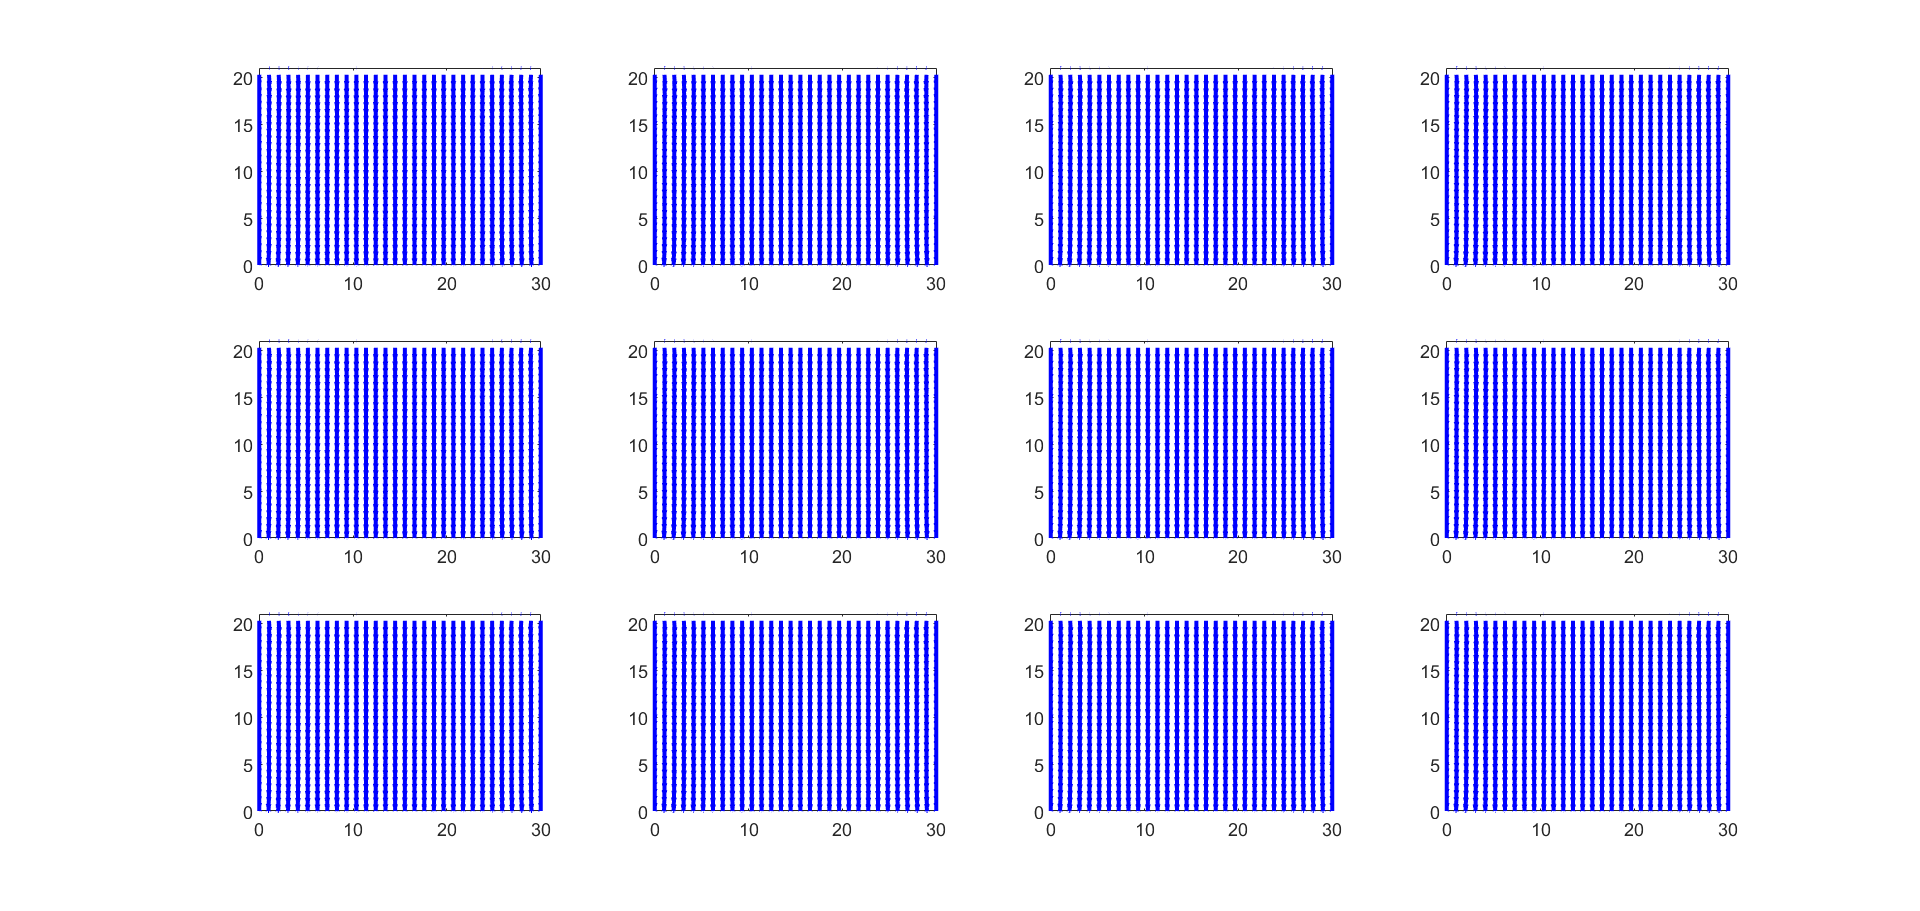
\includegraphics[scale=0.35]{C3.png}
%	\caption{Time-independent; Optimal Control for $a = 0.01$} 
%	\label{F8a}
%\end{figure}
%
%We wanted to see whether the time independent flow control is similar to the $\nabla V_{ext}$ of the target.
%The target state was influenced by $V_{ext} = 0.1 y_2$. The forward state for the OCP was influenced by $V_{ext} = 0.01 y_2$. 
%Figure \ref{F1a} shows the control and $\nabla V_{ext}$ of the target. We can see that one of these is positive, while the other one is negative. This is due to the opposite signs of $\w$ and $\nabla V_{ext}$ in the PDE.
%
%\begin{figure}[h]
%	\centering
%	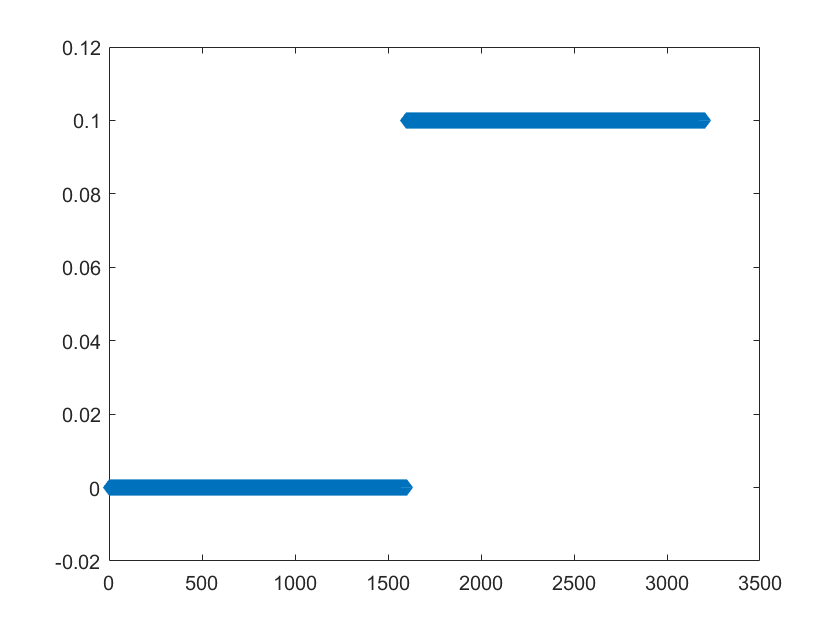
\includegraphics[scale=0.35]{V1.png}
%	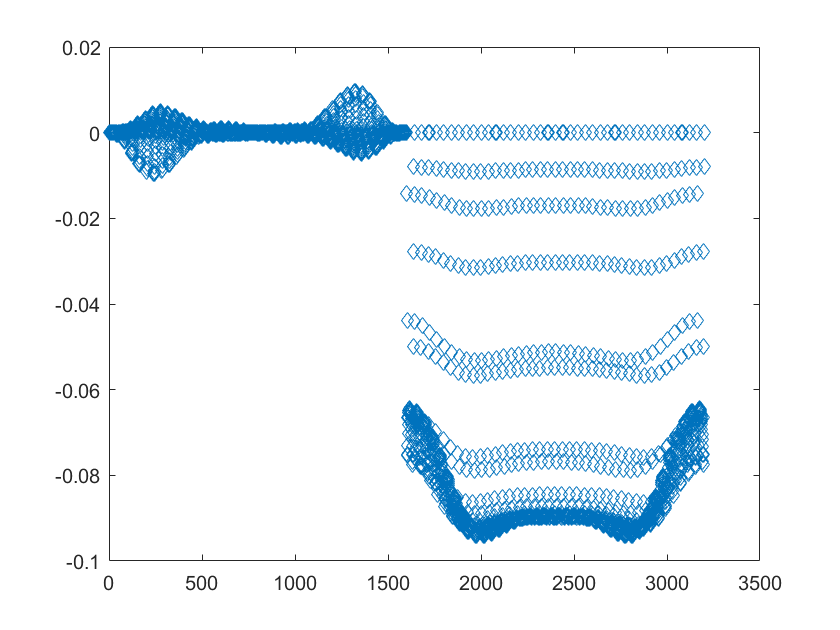
\includegraphics[scale=0.35]{W1.png}
%	\caption{$\nabla V_{ext}$ of target and optimal control $\w$.} 
%	\label{F1a}
%\end{figure}

\subsubsection{Optimization in a Periodic Box}
\subsubsection{Optimization in a Periodic Box - Time-Independent Control}

\subsubsection{Optimization in a Multishape}
\subsubsection{Optimization in a Multishape - Time-Independent Control}


\pagebreak	
\bibliography{GeneralBib}
\bibliographystyle{unsrt}




\end{document}